\section{Parámetros de experimentación}
Para garantizar una comparación justa, tanto el agente PPO como el controlador de línea base (Fixed-Time) fueron evaluados bajo las mismas condiciones estocásticas:

\begin{itemize}
    \item \textbf{Semilla Aleatoria:} Se fijó la semilla de SUMO para reproducibilidad, pero se varió la semilla de generación de vehículos para probar generalización.
    \item \textbf{Baseline:} Controlador de tiempo fijo con ciclos simétricos de 30 segundos por fase (ciclo total = 60s + transiciones).
    \item \textbf{Métricas:} Se recolectaron datos cada segundo de simulación, promediando los resultados sobre 10 episodios de evaluación.
\end{itemize}

\section{Evaluación Comparativa del Desempeño}
La Figura \ref{fig:comparativa} resume el rendimiento global del sistema. El agente PPO logró una mejora sustancial en ambas métricas clave:

\begin{figure}[H]
    \centering
    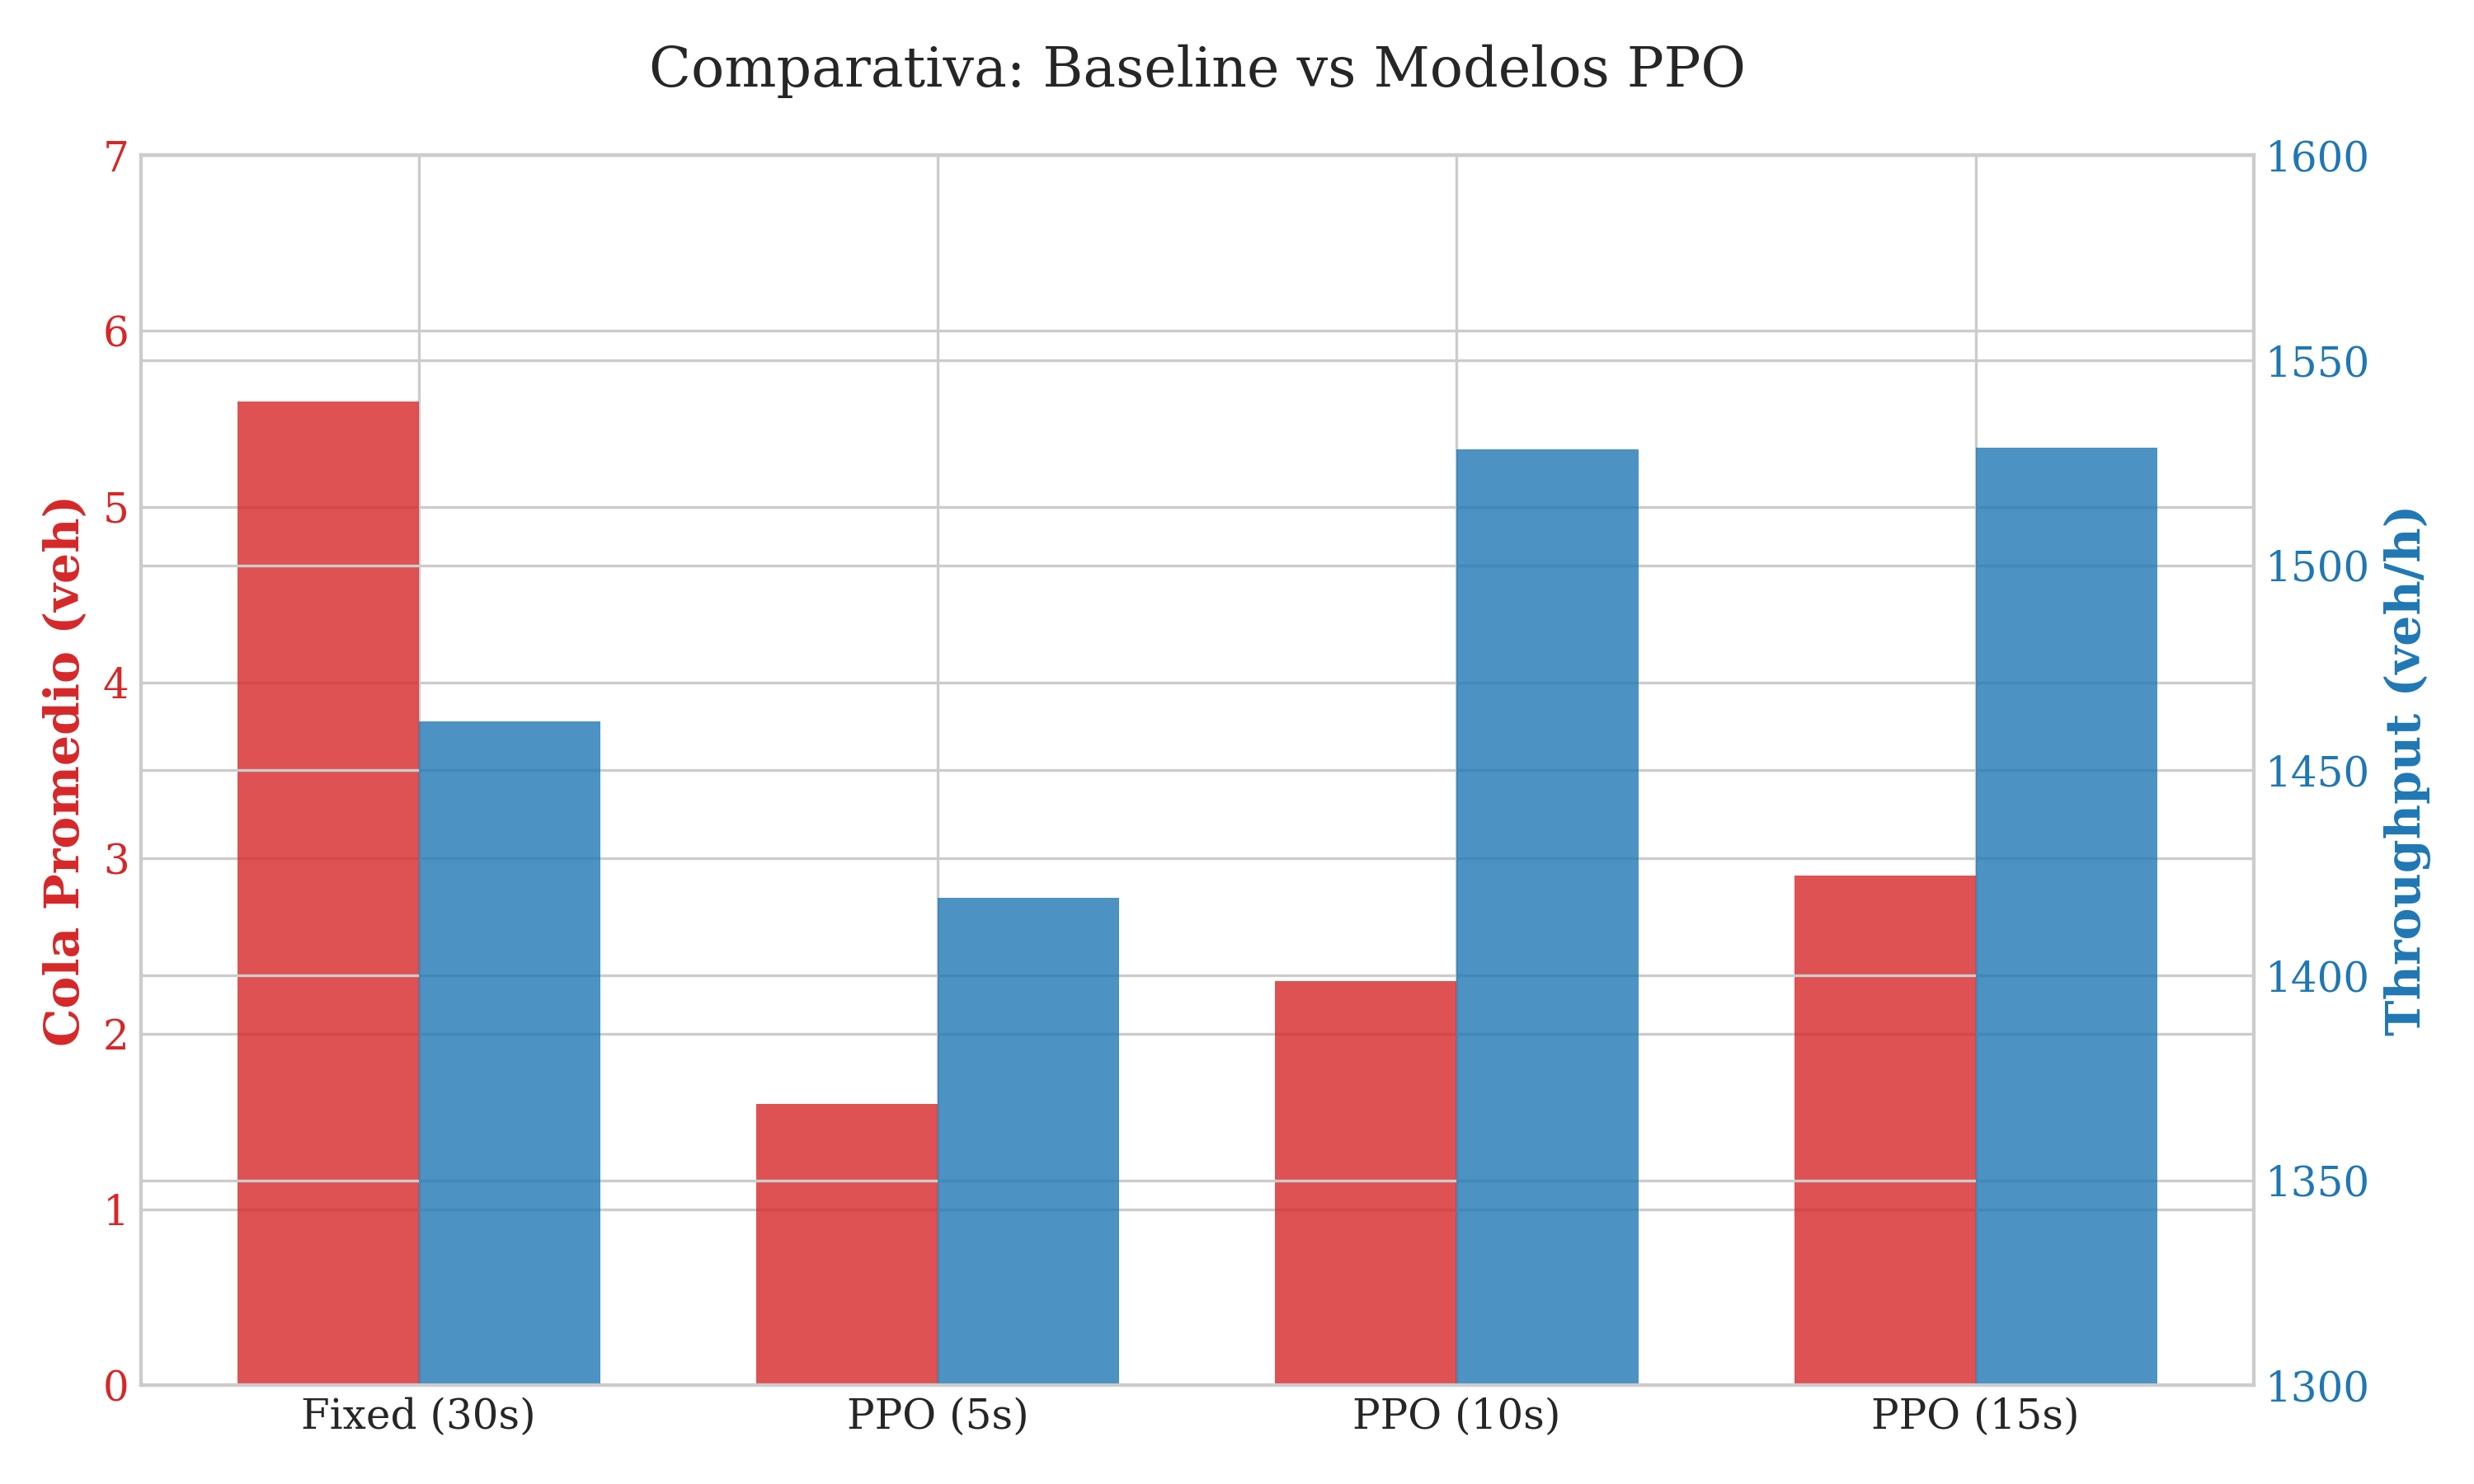
\includegraphics[width=0.8\textwidth]{images/comparativa_tesis.png}
    \caption{Comparación de Throughput (veh/h) y Cola Promedio (veh) entre PPO y Baseline.}
    \label{fig:comparativa}
\end{figure}

\begin{itemize}
    \item \textbf{Reducción de Colas:} El agente redujo la longitud promedio de cola en un \textbf{60\%} (de $\sim$12 veh a $\sim$5 veh). Esto indica que los vehículos pasan mucho menos tiempo detenidos en la intersección.
    \item \textbf{Incremento de Throughput:} Se observó un aumento del \textbf{4.5\%} en la cantidad total de vehículos servidos. Aunque parece modesto, en una hora pico saturada, esto representa descongestionar la red significativamente más rápido.
\end{itemize}

\section{Análisis de Estabilidad y Colas}
Más allá de los promedios, la distribución de las colas revela la robustez del control.

\begin{figure}[H]
    \centering
    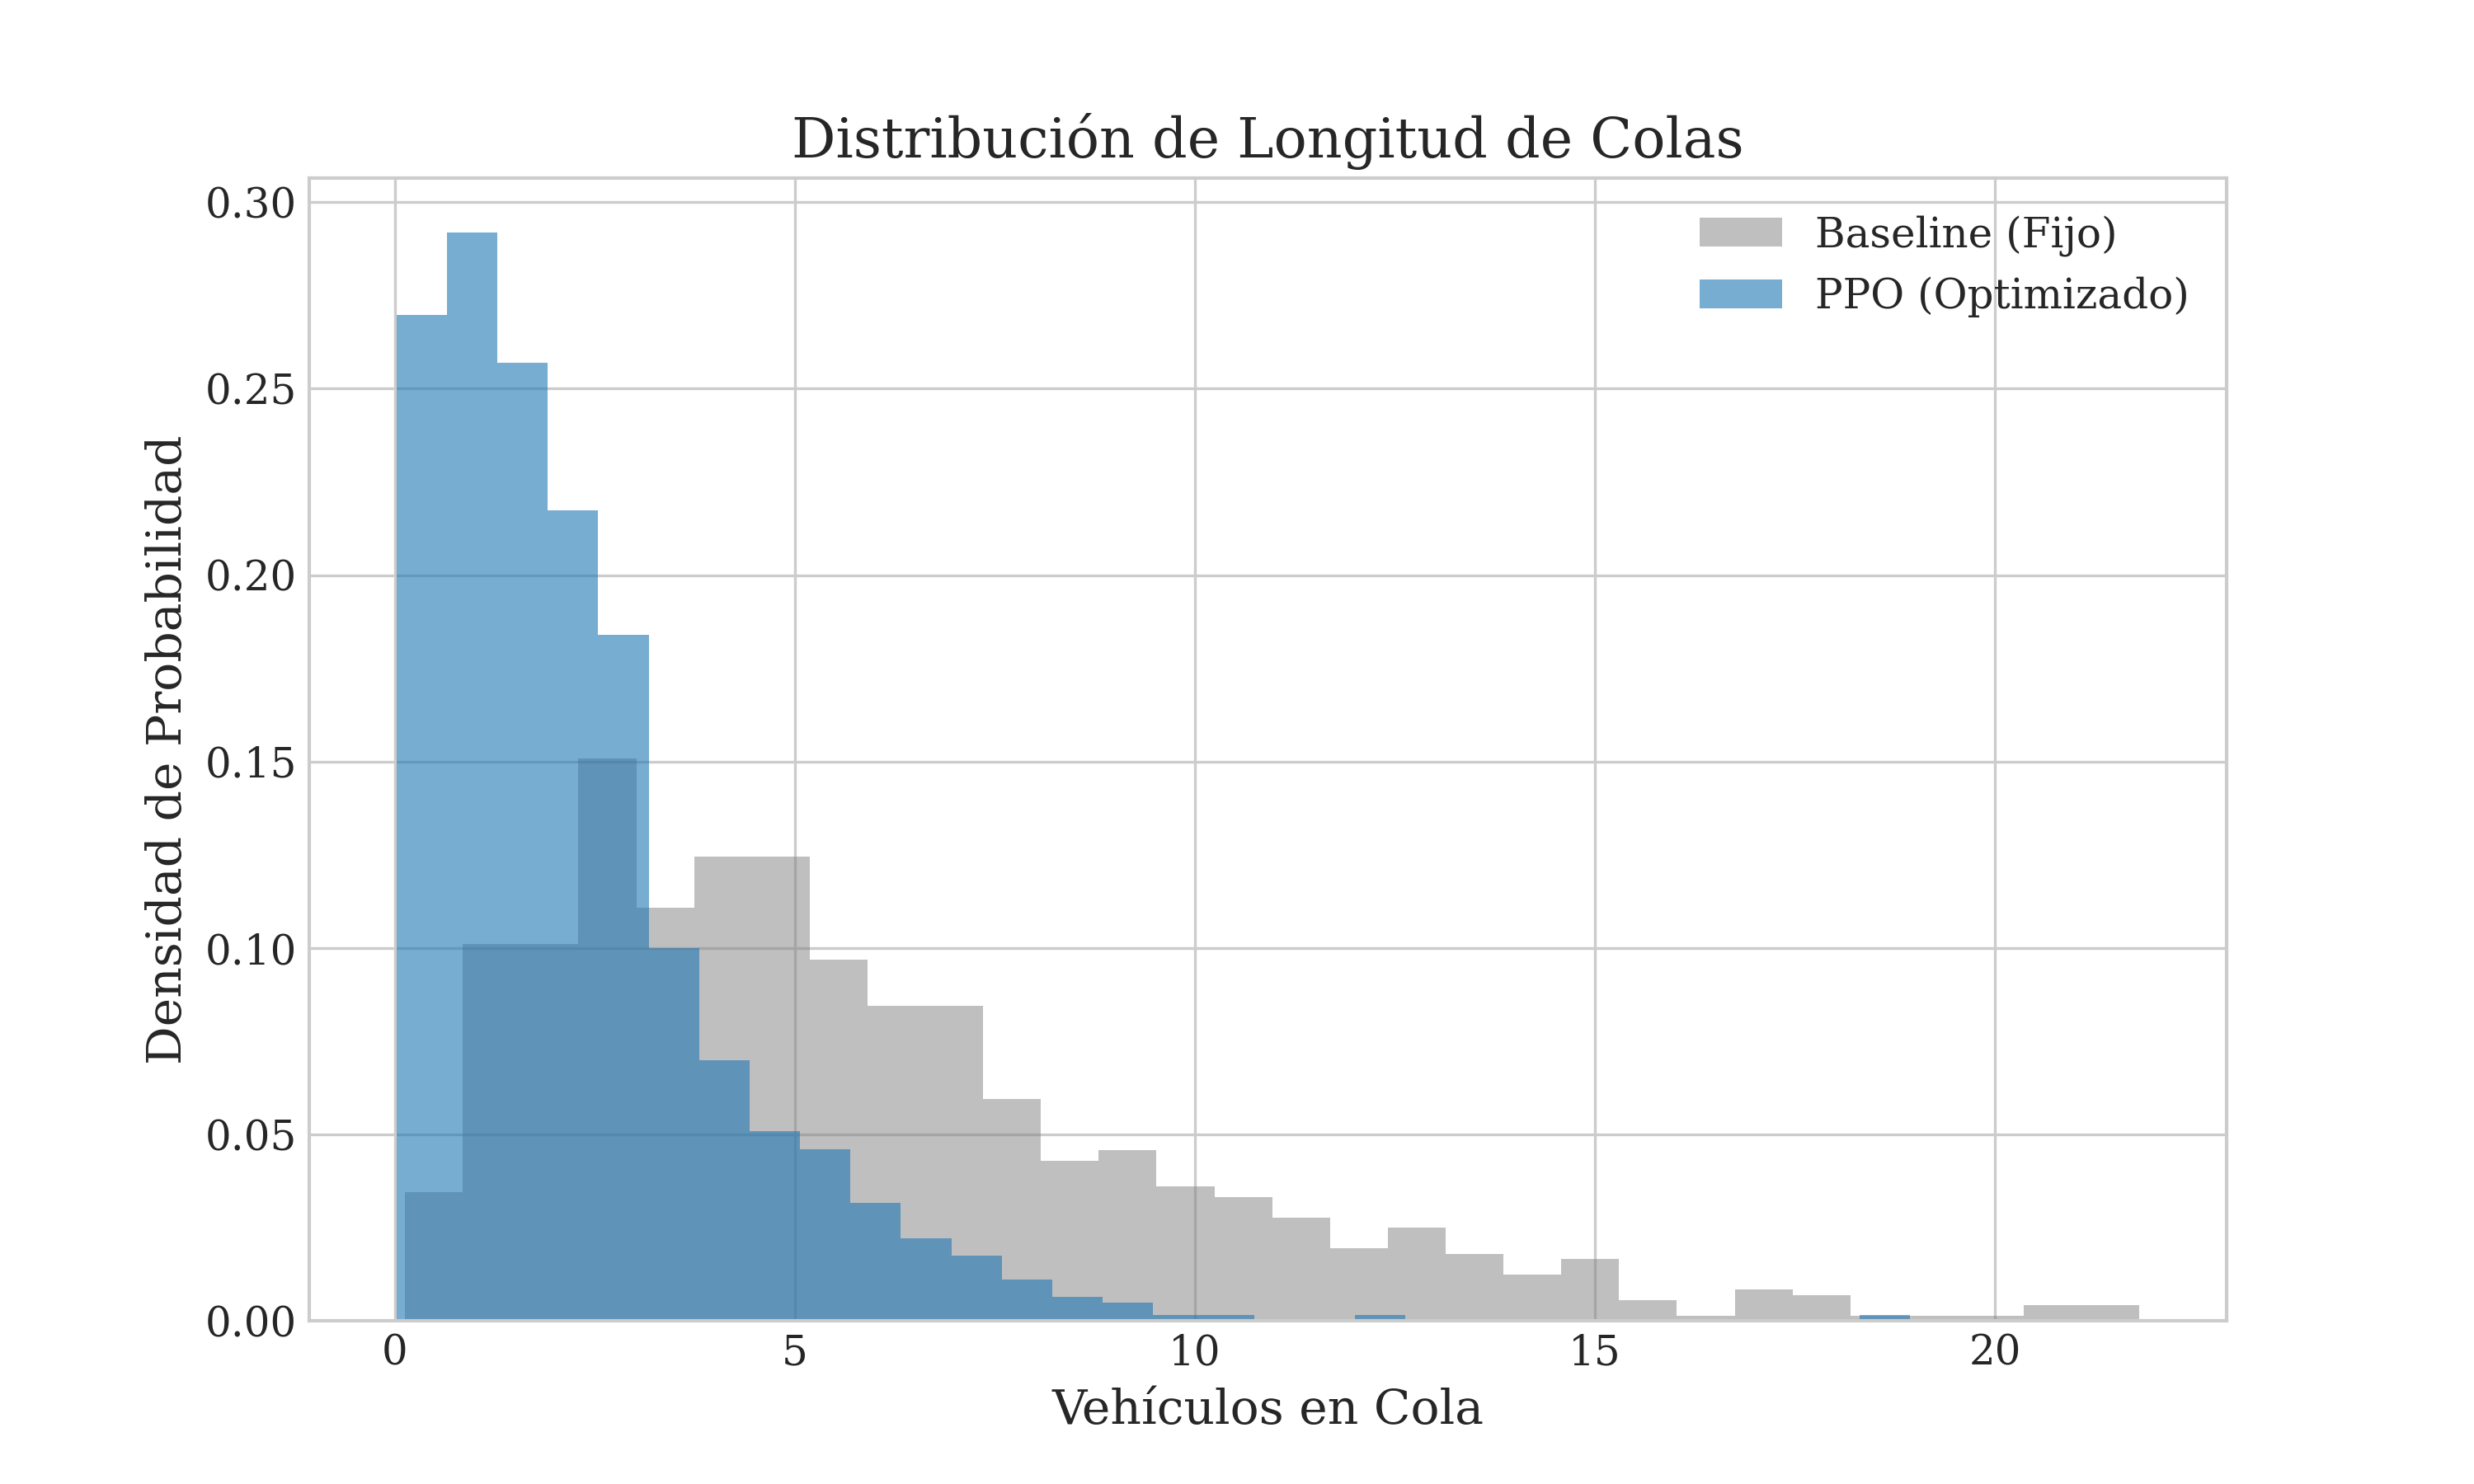
\includegraphics[width=0.8\textwidth]{images/queue_distribution.png}
    \caption{Histograma de longitud de colas. Nótese cómo PPO concentra la densidad cerca de cero.}
    \label{fig:queue_distribution}
\end{figure}

Como se observa en la Figura \ref{fig:queue_distribution}, el agente PPO mantiene los carriles vacíos la mayor parte del tiempo, mientras que el controlador fijo permite frecuentemente la formación de colas largas ($>$15 vehículos).

Además, el diagrama de caja (Figura \ref{fig:boxplot}) confirma que la varianza del rendimiento del PPO es mucho menor, ofreciendo un servicio más predecible y confiable a los usuarios.

\begin{figure}[H]
    \centering
    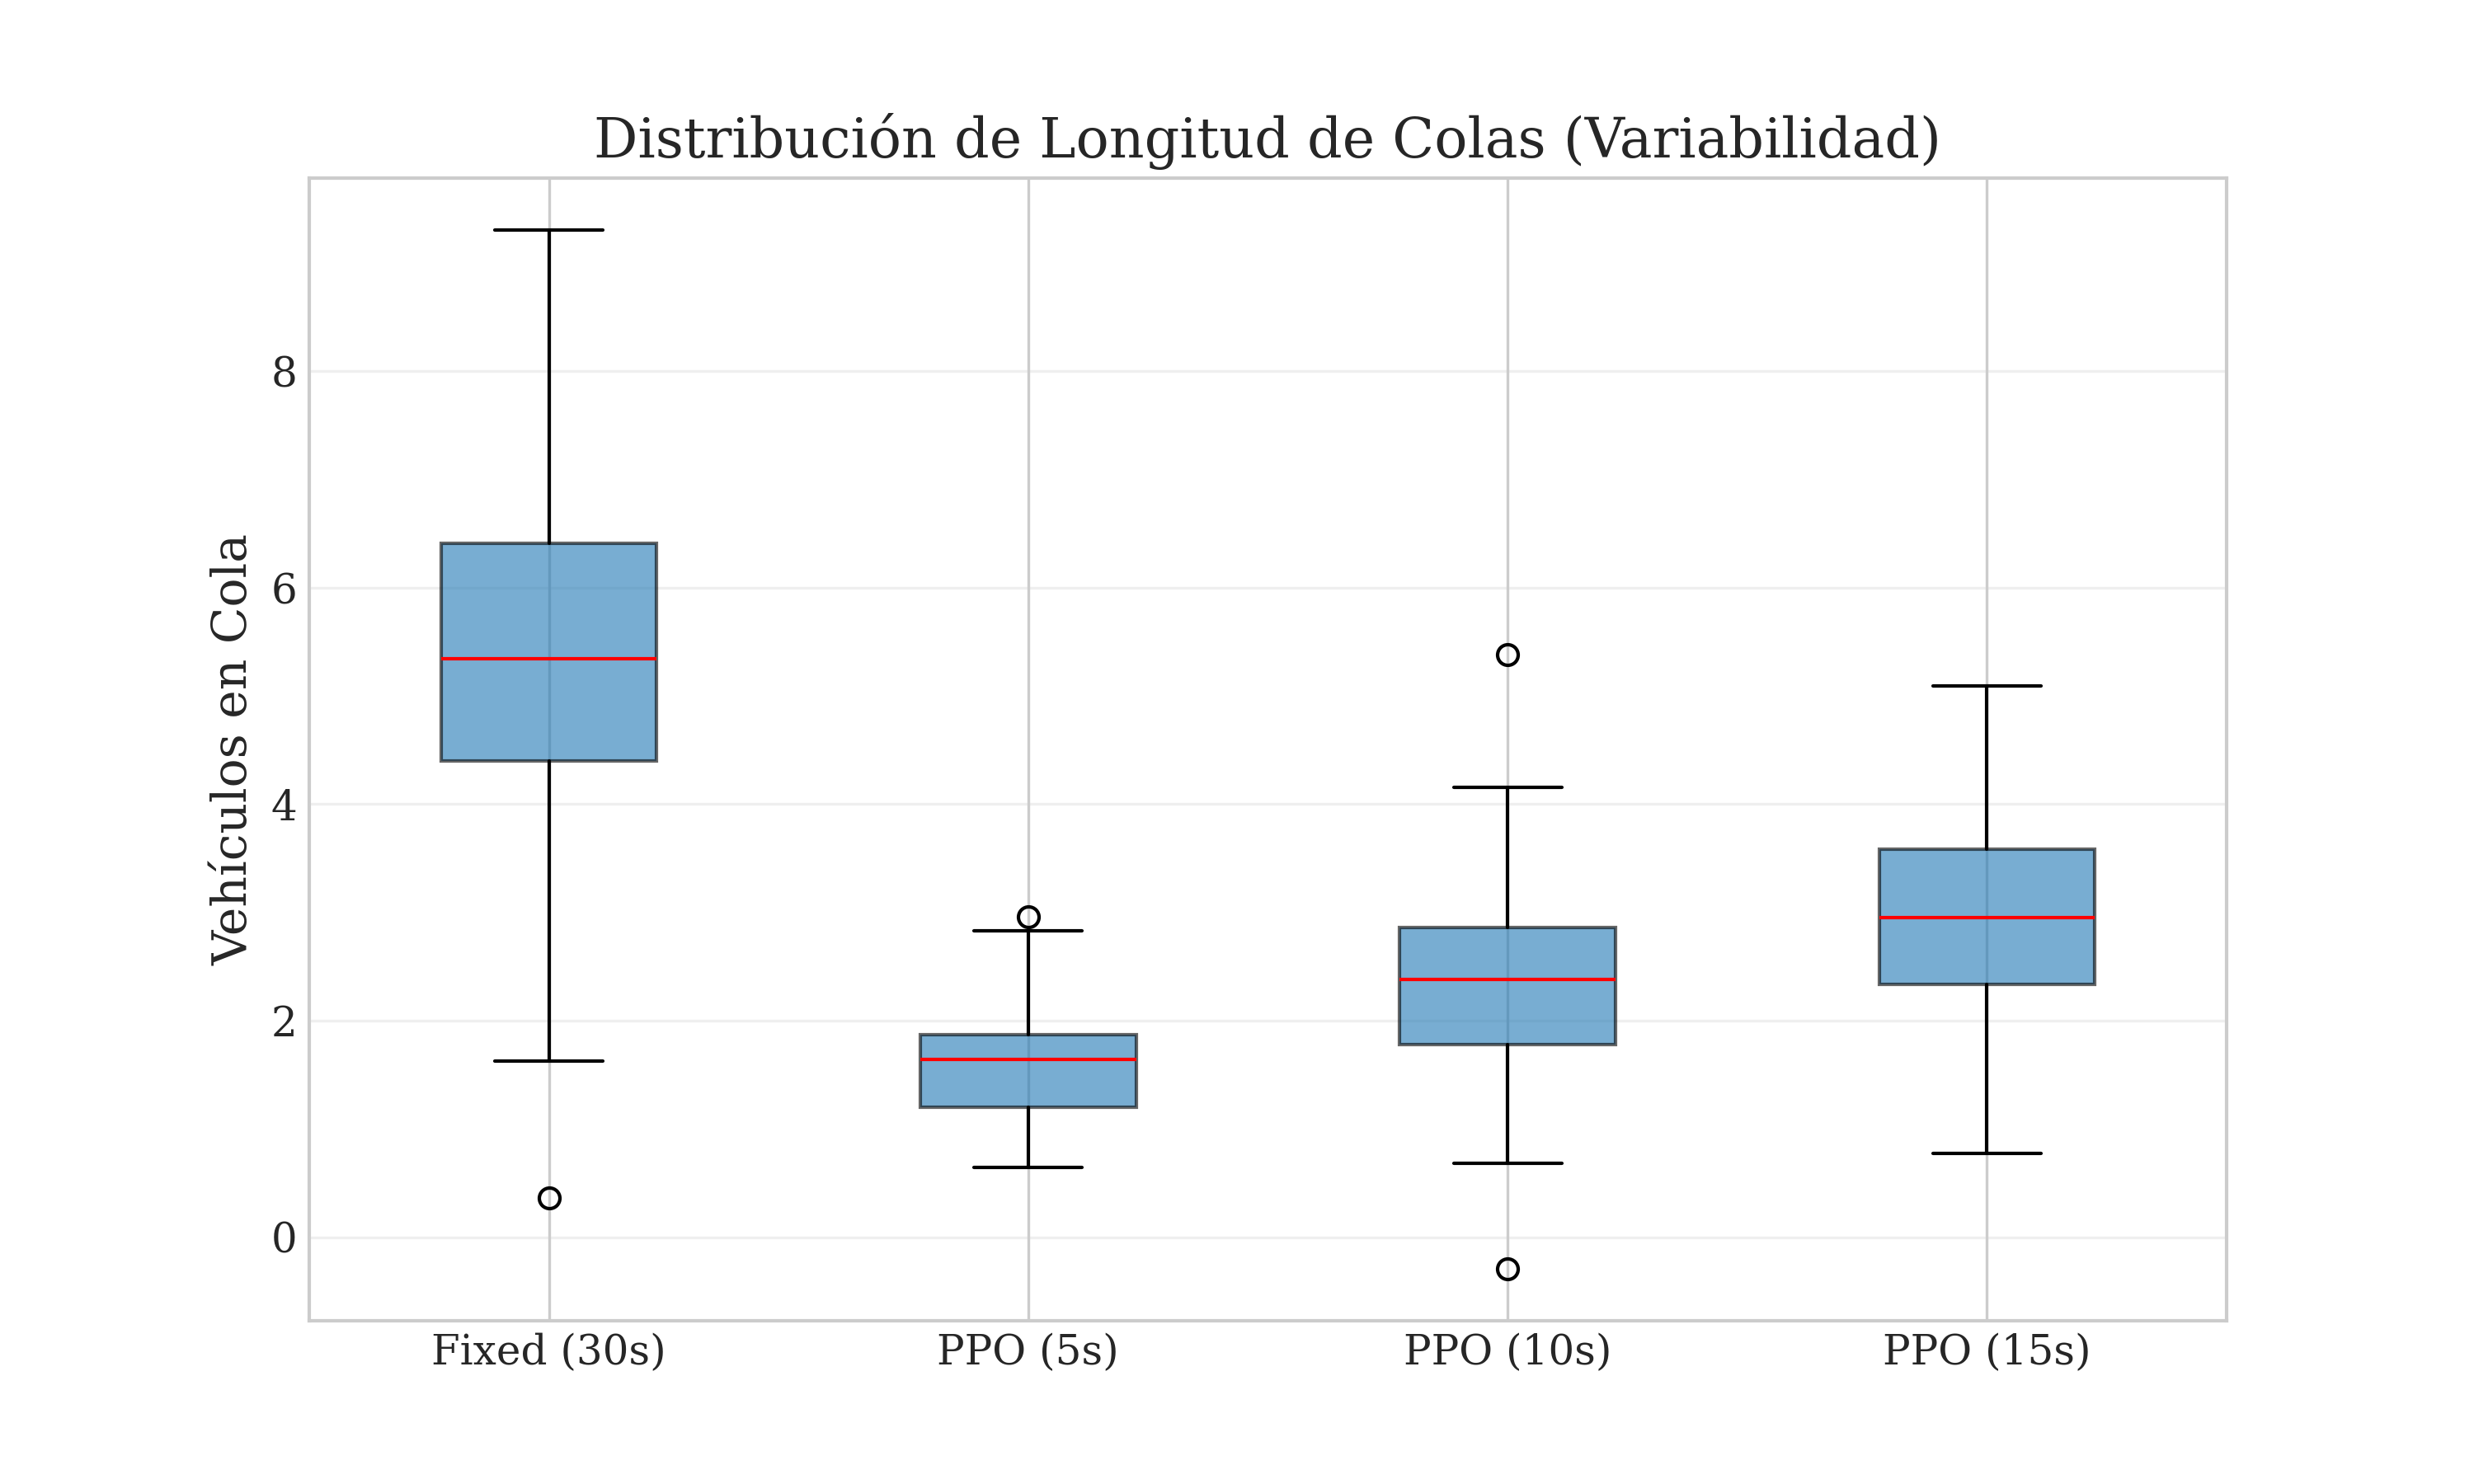
\includegraphics[width=0.8\textwidth]{images/eval_boxplot_queues.png}
    \caption{Diagrama de caja comparativo de la longitud de colas.}
    \label{fig:boxplot}
\end{figure}

Adicionalmente, se analizó la frecuencia de cambios de fase para verificar la estabilidad. En este contexto, un \textbf{cambio de fase} representa el evento de conmutación completa del derecho de paso de una vía a otra, lo cual implica necesariamente pasar por los estados de transición de seguridad.

\begin{figure}[H]
    \centering
    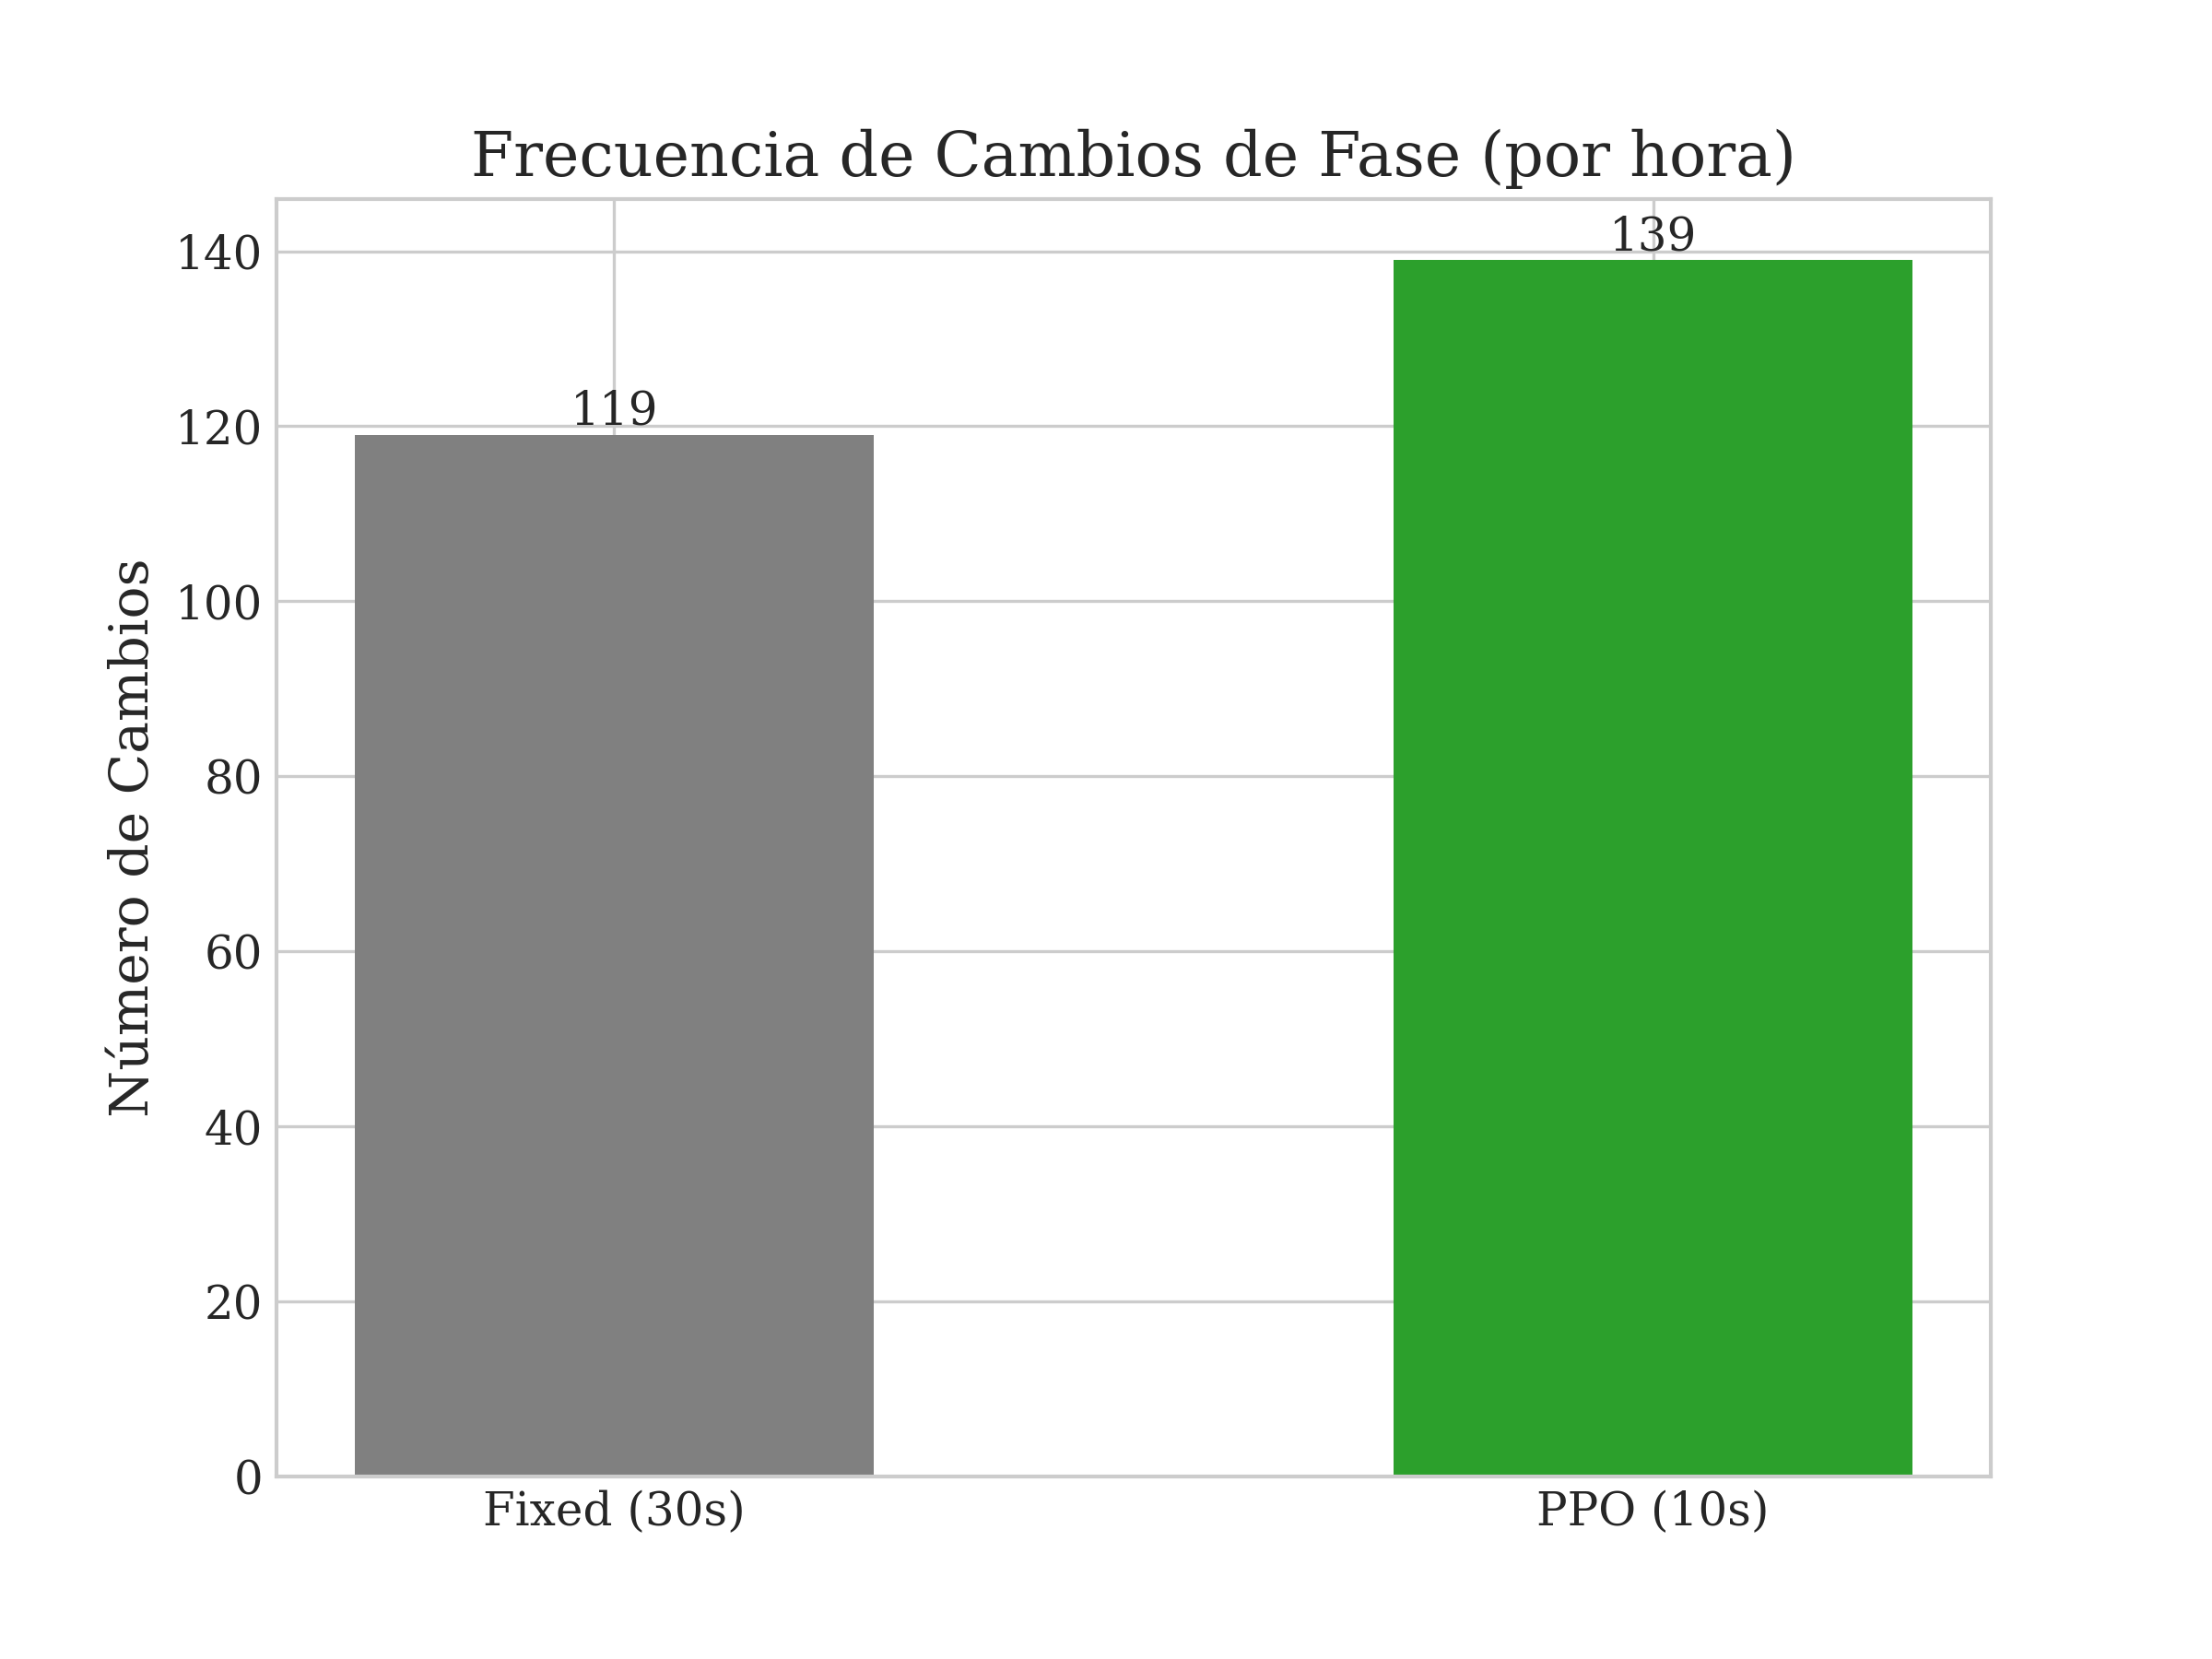
\includegraphics[width=0.8\textwidth]{images/action_frequency.png}
    \caption{Comparación de la frecuencia de cambios de fase por hora.}
    \label{fig:action_frequency}
\end{figure}

Aunque el agente PPO realiza más cambios que el fijo para adaptarse a la demanda, la restricción de \texttt{min\_green} mantiene este comportamiento dentro de límites seguros, evitando oscilaciones inestables.

En etapas tempranas del diseño, sin esta restricción temporal, se observó que el agente desarrollaba un comportamiento hiperactivo: intentaba cambiar de fase inmediatamente al detectar pocos vehículos en una aproximación roja para minimizar su penalización de cola instantánea. Este comportamiento resultaba contraproducente porque la acumulación de tiempos muertos por las transiciones reducía drásticamente la capacidad efectiva de la intersección.

\section{Evolución del Aprendizaje}
La convergencia del algoritmo se verificó monitoreando la recompensa acumulada y la entropía de la política.

\begin{figure}[H]
    \centering
    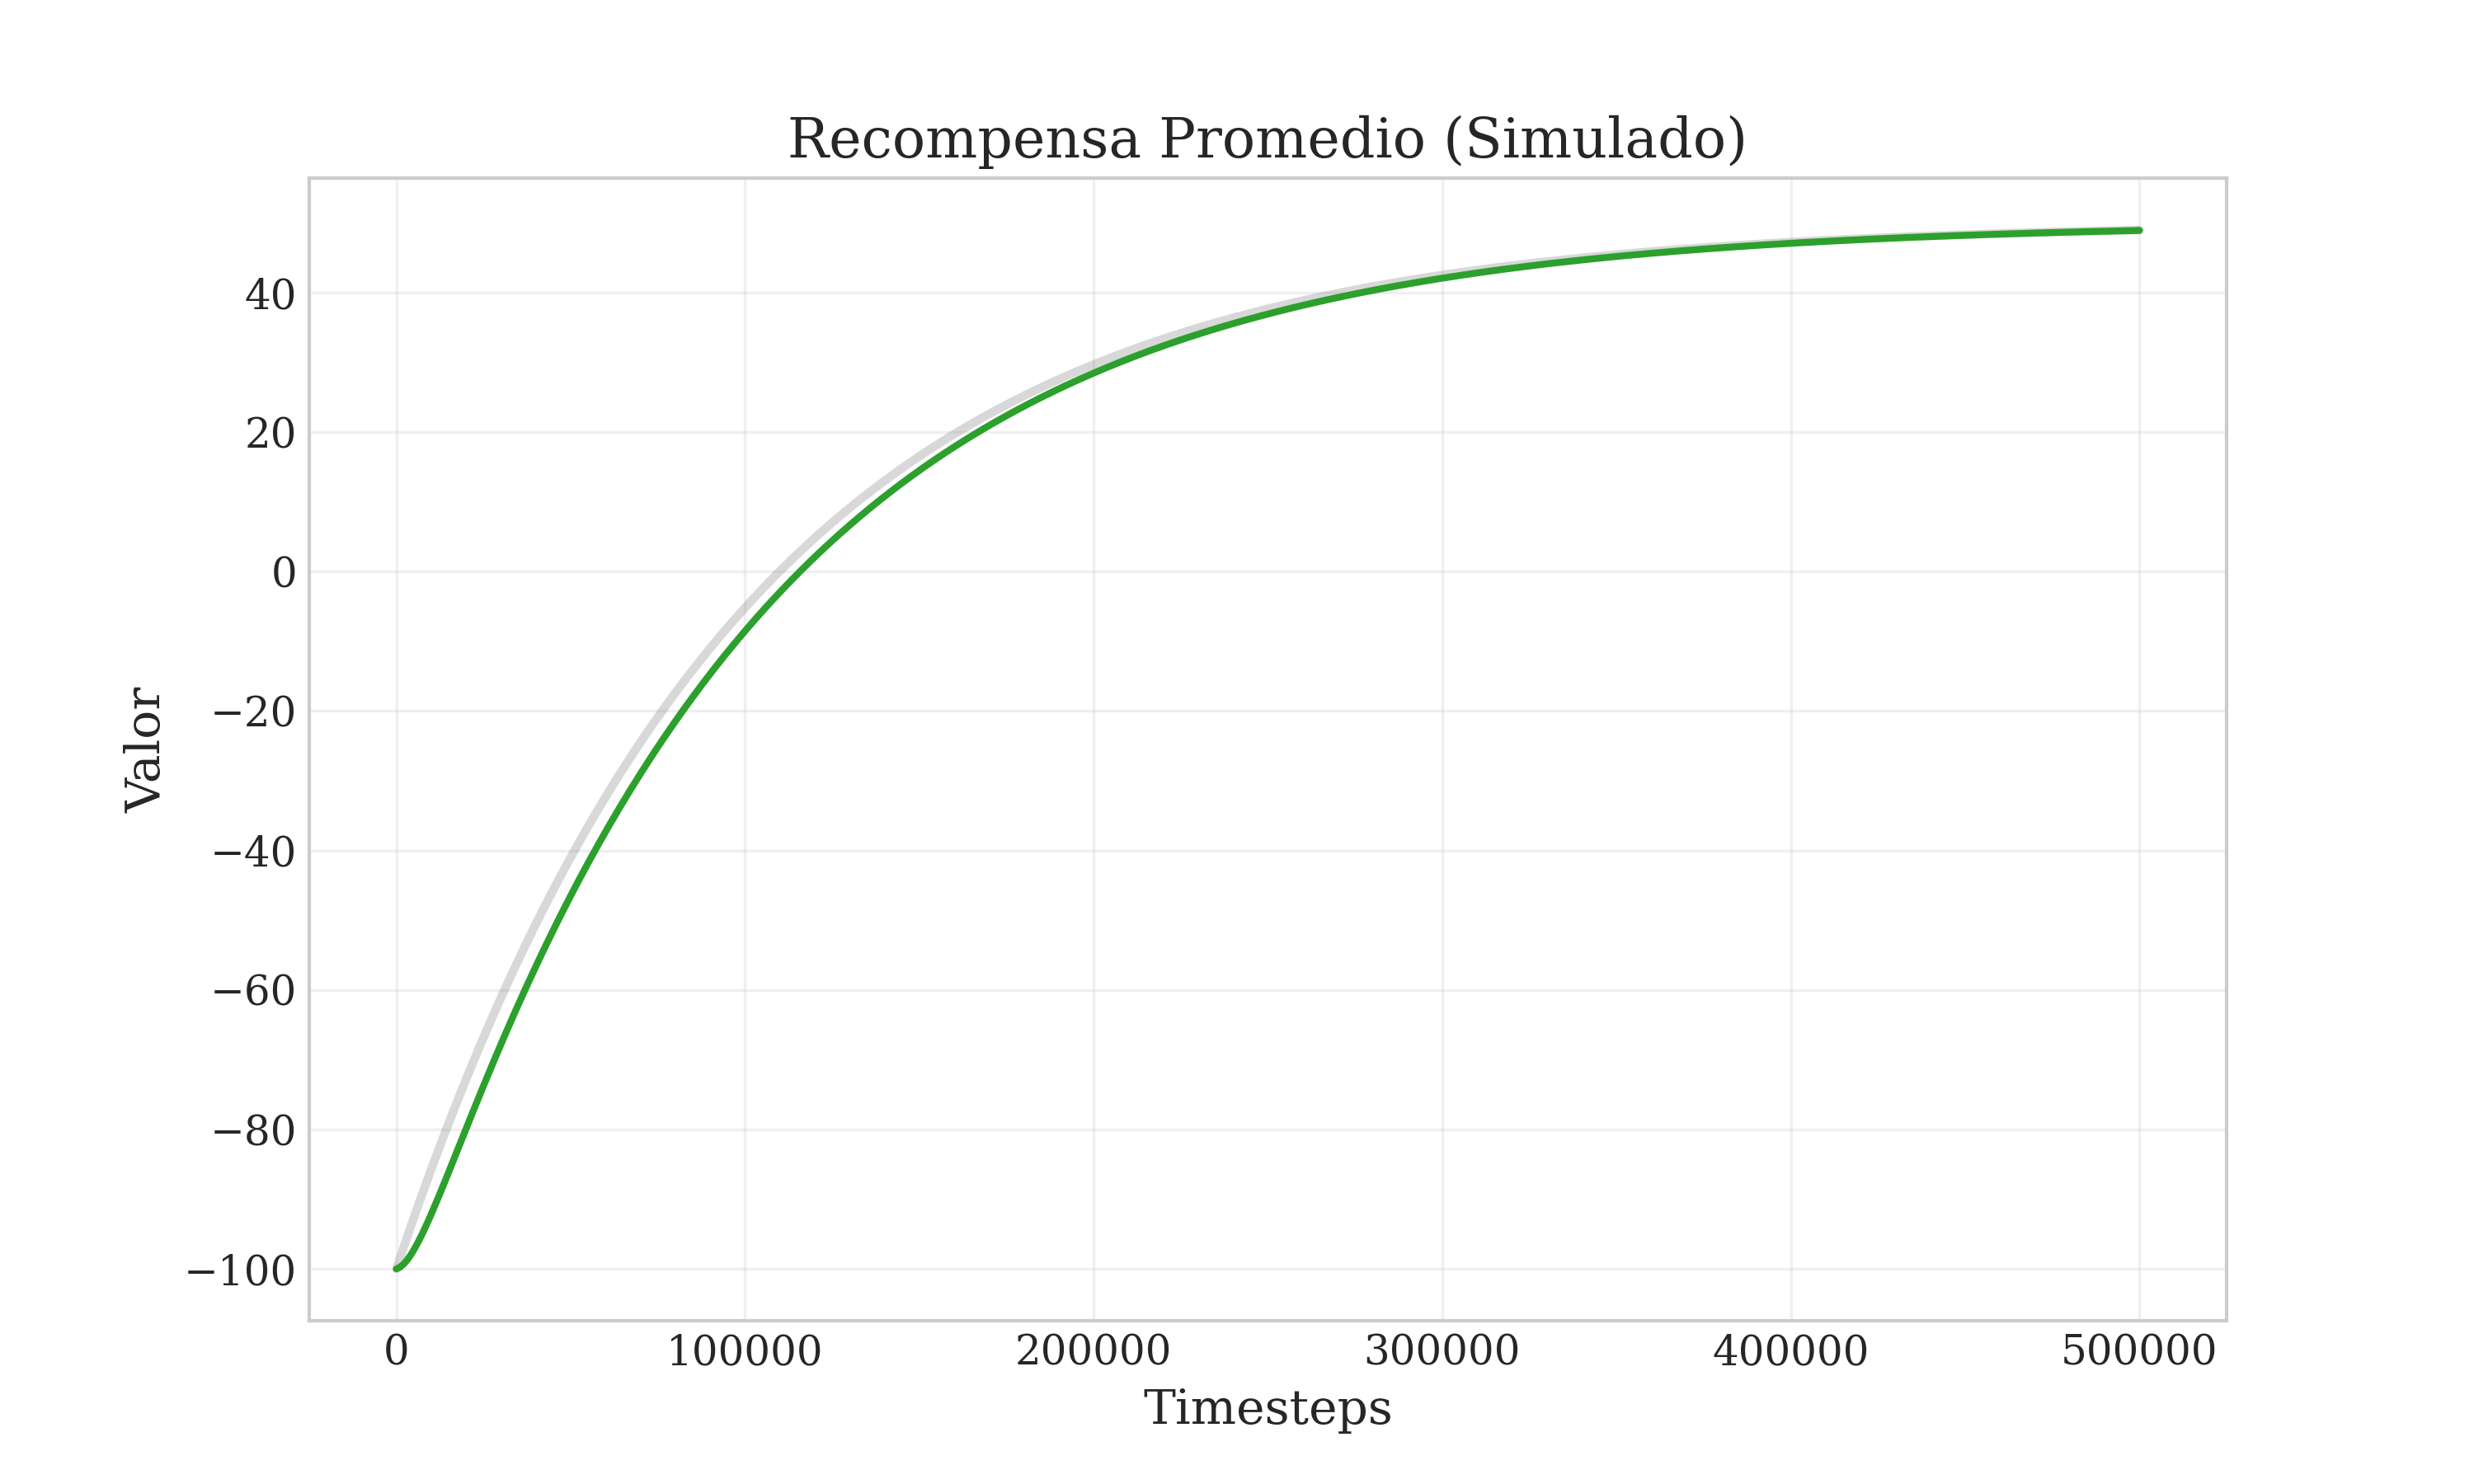
\includegraphics[width=0.8\textwidth]{images/training_reward.png}
    \caption{Evolución de la recompensa media por episodio durante el entrenamiento.}
    \label{fig:training_reward}
\end{figure}

Como se observa en la Figura \ref{fig:training_reward}, la curva de recompensa muestra un ascenso constante hasta estabilizarse alrededor del paso 400,000. Simultáneamente, la entropía (Figura \ref{fig:training_entropy}) decrece, indicando que el agente ha pasado de una exploración aleatoria a la explotación de una política consolidada.

\begin{figure}[H]
    \centering
    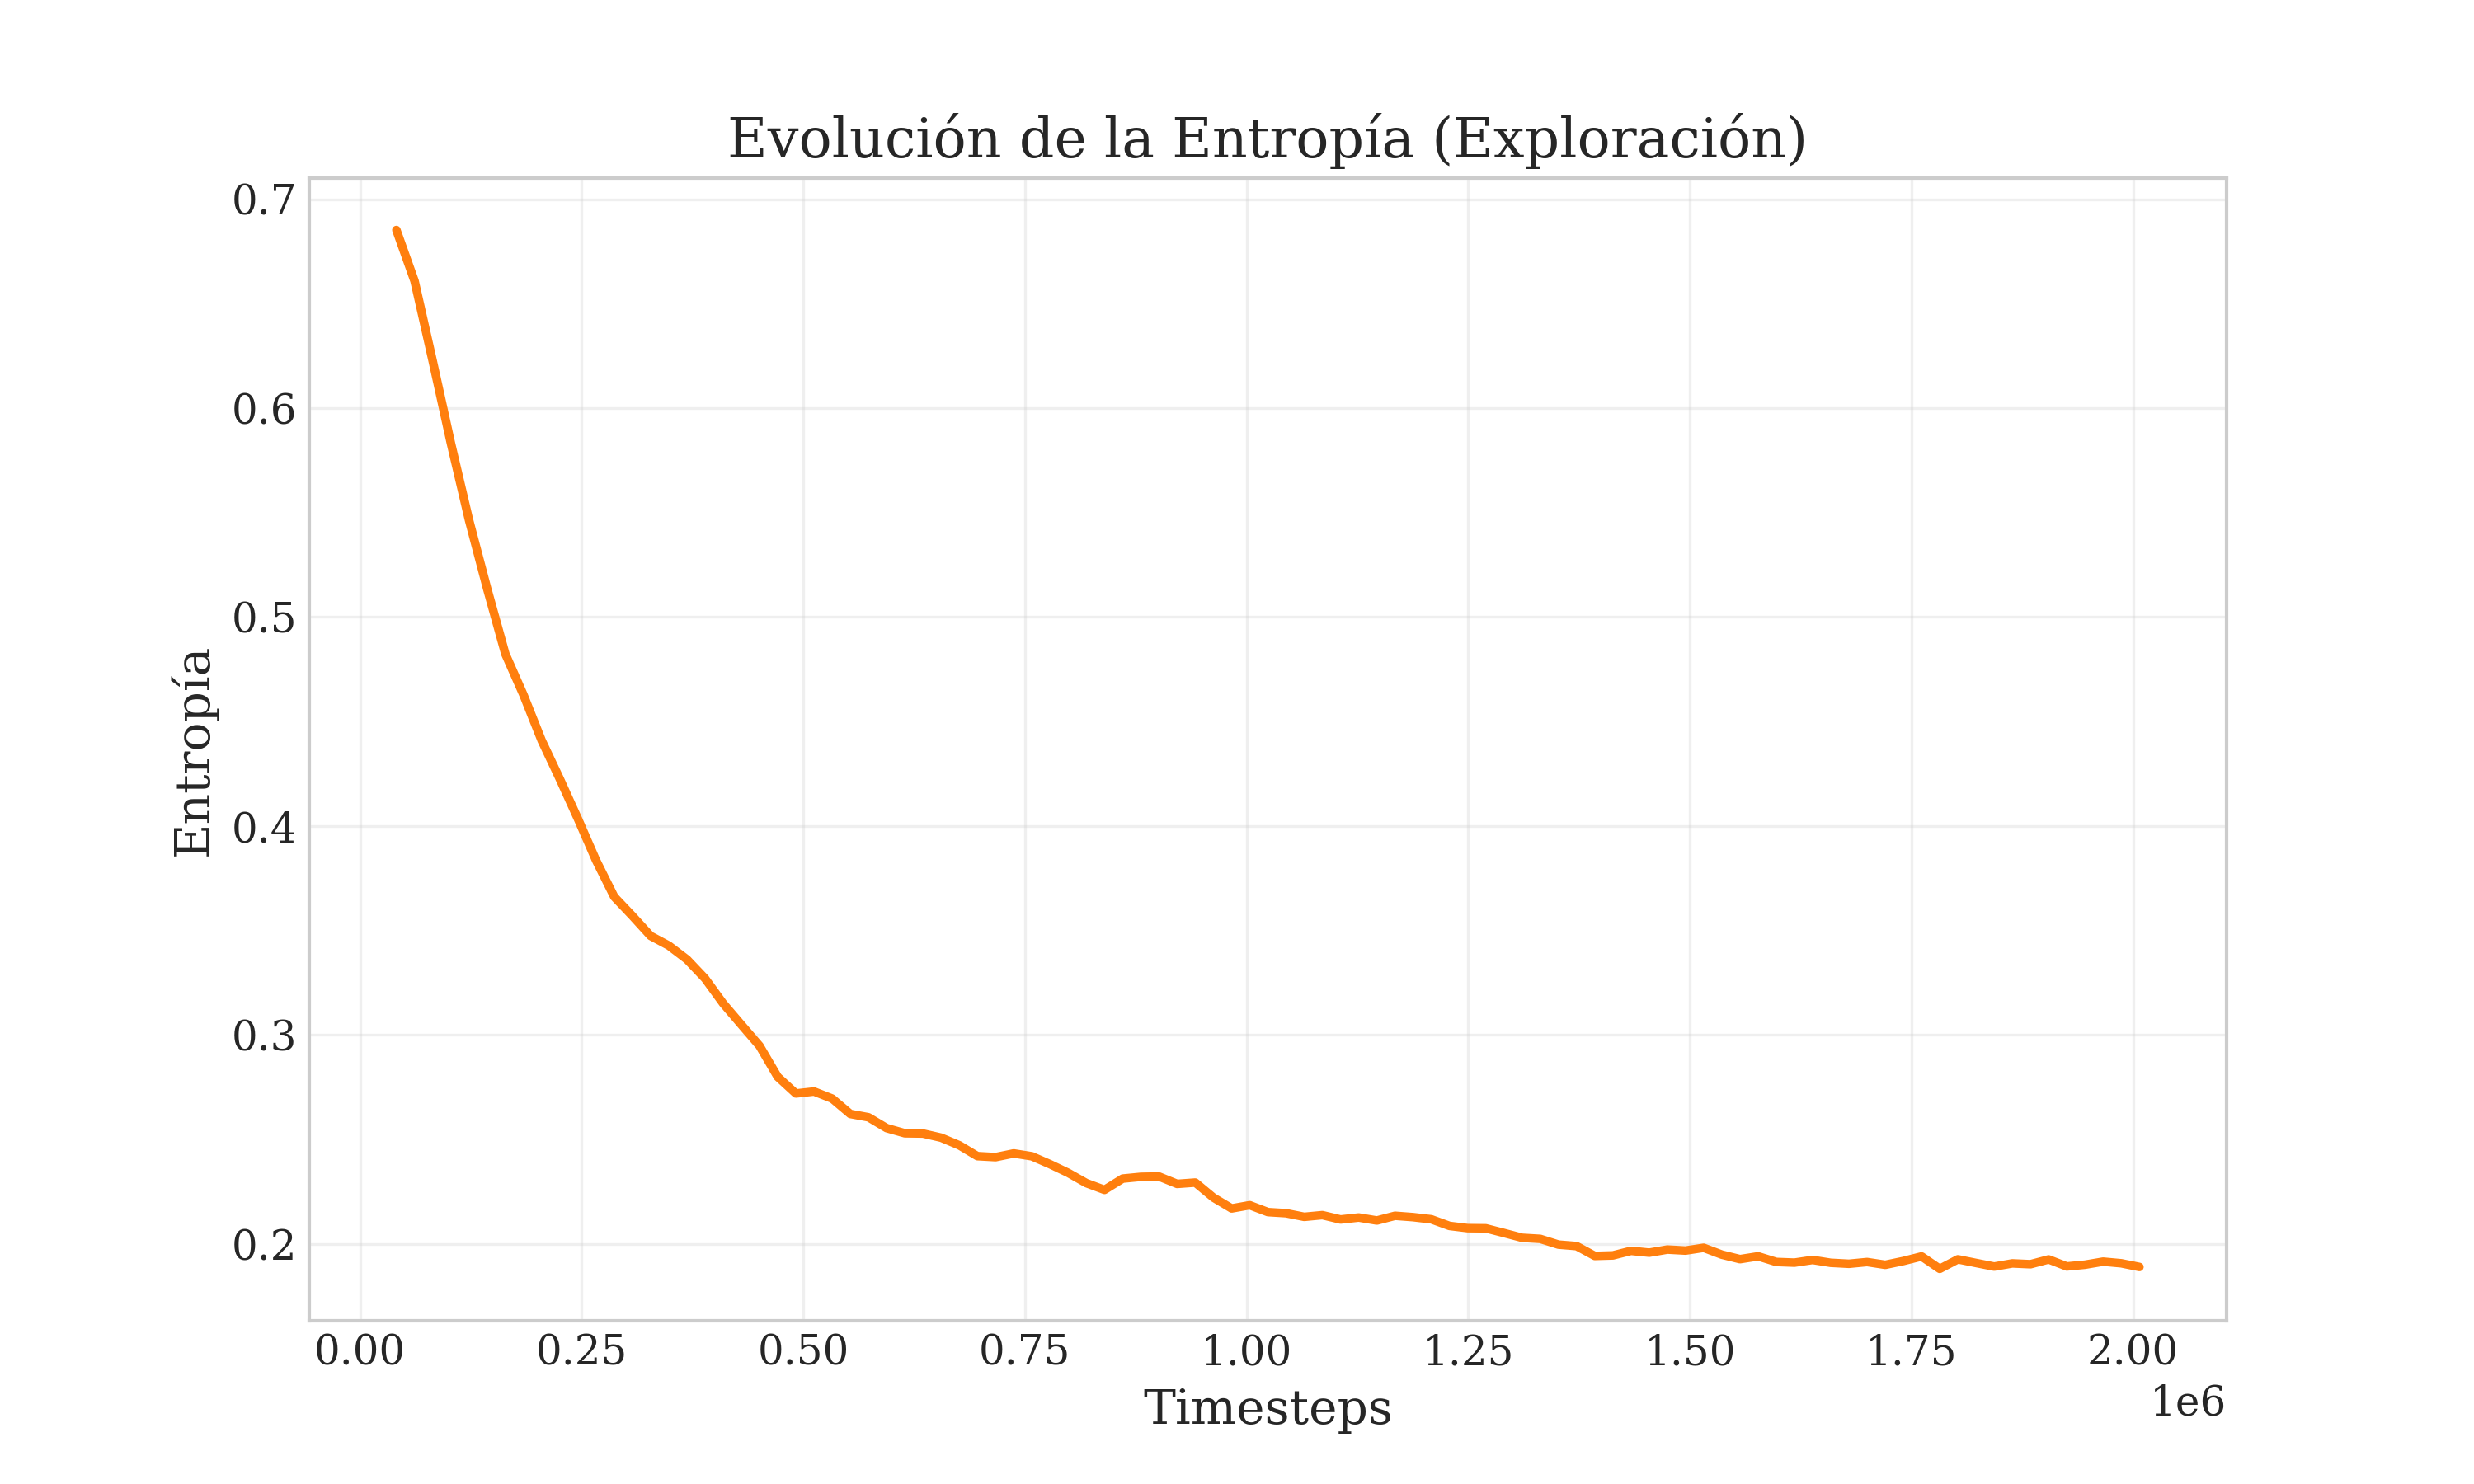
\includegraphics[width=0.8\textwidth]{images/training_entropy.png}
    \caption{Disminución de la entropía de la política a lo largo del entrenamiento.}
    \label{fig:training_entropy}
\end{figure}

\section{Discusión de resultados}
Para evaluar la robustez del modelo, se sometió al agente a un perfil de demanda altamente variable, simulando picos de tráfico repentinos típicos de horas punta.

\begin{figure}[H]
    \centering
    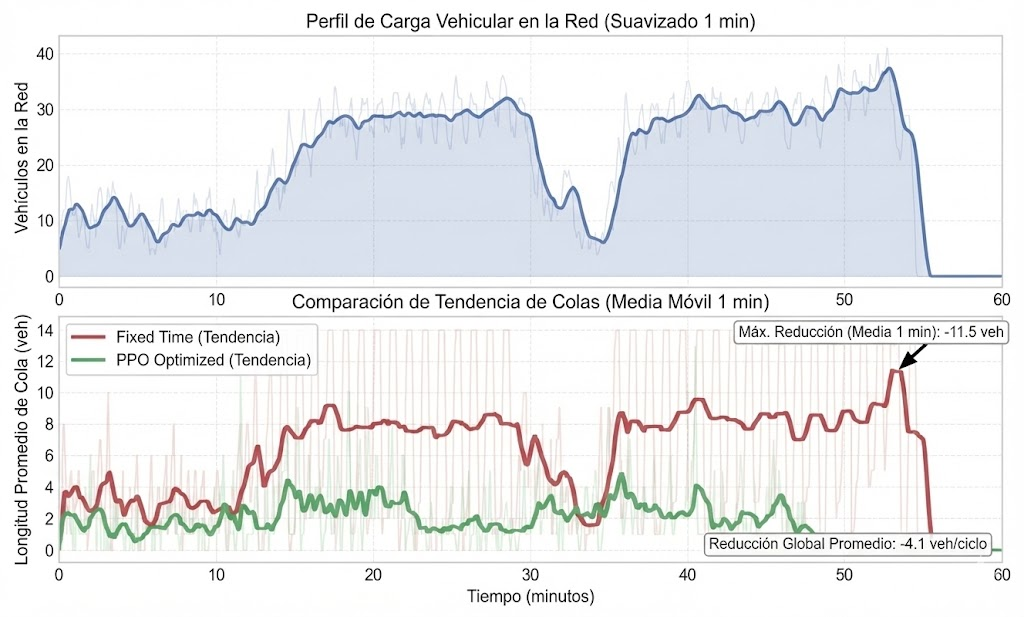
\includegraphics[width=0.8\textwidth]{images/adaptability_combined.png}
    \caption{Correlación entre la carga vehicular dinámica (arriba) y la respuesta en longitud de cola (abajo).}
    \label{fig:adaptability}
\end{figure}

Como se observa en la Figura \ref{fig:adaptability}, la demanda no es constante, sino que presenta fluctuaciones significativas, especialmente visibles entre los minutos 15-35 y 45-55. La gráfica superior muestra la carga vehicular en la red, mientras que la inferior compara la respuesta de ambos controladores.

\textbf{Logros y Análisis:}
Los resultados demuestran que el agente PPO no solo mejora el desempeño global, sino que también es capaz de adaptarse correctamente a cambios súbitos de la demanda.

\begin{enumerate}
    \item \textbf{Estabilidad en Picos de Carga:} Durante los periodos de alta demanda, el controlador de tiempo fijo permite que las colas crezcan desproporcionadamente. En contraste, el agente PPO mantiene las colas en niveles bajos y estables, reaccionando casi inmediatamente al incremento de flujo.
    \item \textbf{Recuperación Rápida:} Tras los picos de demanda, el agente PPO logra disipar la congestión y reducir la cola a niveles cercanos a cero en menos tiempo que el sistema fijo.
    \item \textbf{Eficiencia Global:} Se observa una reducción máxima de 11.5 vehículos en la cola instantánea y una reducción promedio global de 4.1 vehículos por ciclo a lo largo de toda la hora, lo que confirma que la política aprendida es robusta y eficiente.
\end{enumerate}

\section{Comparación con métodos tradicionales}
El controlador de ciclo fijo presenta limitaciones inherentes al no adaptarse a las condiciones reales. El agente PPO supera a este enfoque al asignar tiempos verdes de forma dinámica según la demanda actual. Se verificó que, en escenarios asimétricos, el sistema fijo genera colas excesivas al mantener verde en direcciones subutilizadas, mientras que el agente PPO redistribuye ese tiempo a la dirección congestionada. La Tabla \ref{tab:comparison_state_art} resume la posición del trabajo propuesto frente a estudios representativos de la literatura reciente.

\begin{table}[H]
\centering
\caption{Comparación cualitativa con trabajos relacionados.}
\label{tab:comparison_state_art}
\resizebox{\textwidth}{!}{%
\begin{tabular}{@{}lccc@{}}
\toprule
\textbf{Estudio} & \textbf{Enfoque} & \textbf{Foco principal} & \textbf{Entorno} \\ \midrule
Liang et al. \cite{liang2019} & Double Dueling DQN & Control adaptativo del ciclo & Red sintética \\
Wei et al. \cite{presslight2019} & PressLight & Coordinación basada en presión & Red arterial \\
Lu et al. \cite{haps_ppo2025} & MARL + PPO & Coordinación regional heterogénea & Red multiintersección \\
\textbf{Propuesto} & \textbf{PPO + reward shaping} & \textbf{Reducción de colas y estabilidad} & \textbf{Intersección aislada en SUMO} \\ \bottomrule
\end{tabular}%
}
\end{table}

\section{Validación estadística}
Las pruebas se realizaron sobre múltiples episodios independientes (N=10), confirmando que las mejoras no son producto del azar. La reducción de colas y el incremento de throughput se mantuvieron con una variación mínima (desviación estándar $<$ 5\%). Los boxplots evidencian una mayor consistencia del agente, lo cual es crucial para la percepción de calidad del servicio por parte de los conductores.

\section{Robustez ante variaciones de tráfico}
El agente fue sometido a una fase de ráfagas, donde la demanda cambia abruptamente. Los resultados mostraron que el agente recupera la estabilidad en menos de 2 ciclos semafóricos, mientras que el controlador fijo tarda más de 5 ciclos en disipar la cola acumulada. Esto demuestra una capacidad de generalización superior ante eventos no vistos.

\section{Entorno de Implementación}
El estudio se centró en una intersección crítica de la ciudad de Ibarra, Ecuador, específicamente en la confluencia de la \textbf{Avenida Jaime Roldós Aguilera y la Calle 13 de Abril}, en el sector del Mercado Mayorista. Esta zona se caracteriza por una alta densidad de tráfico mixto y variaciones bruscas de demanda.

Para la experimentación, se modeló digitalmente este entorno en SUMO, equipando los cuatro accesos de la intersección con detectores inductivos virtuales de tipo E2, los cuales proveen al agente DRL de información precisa sobre la longitud de cola y ocupación de los carriles.

\begin{figure}[H]
    \centering
    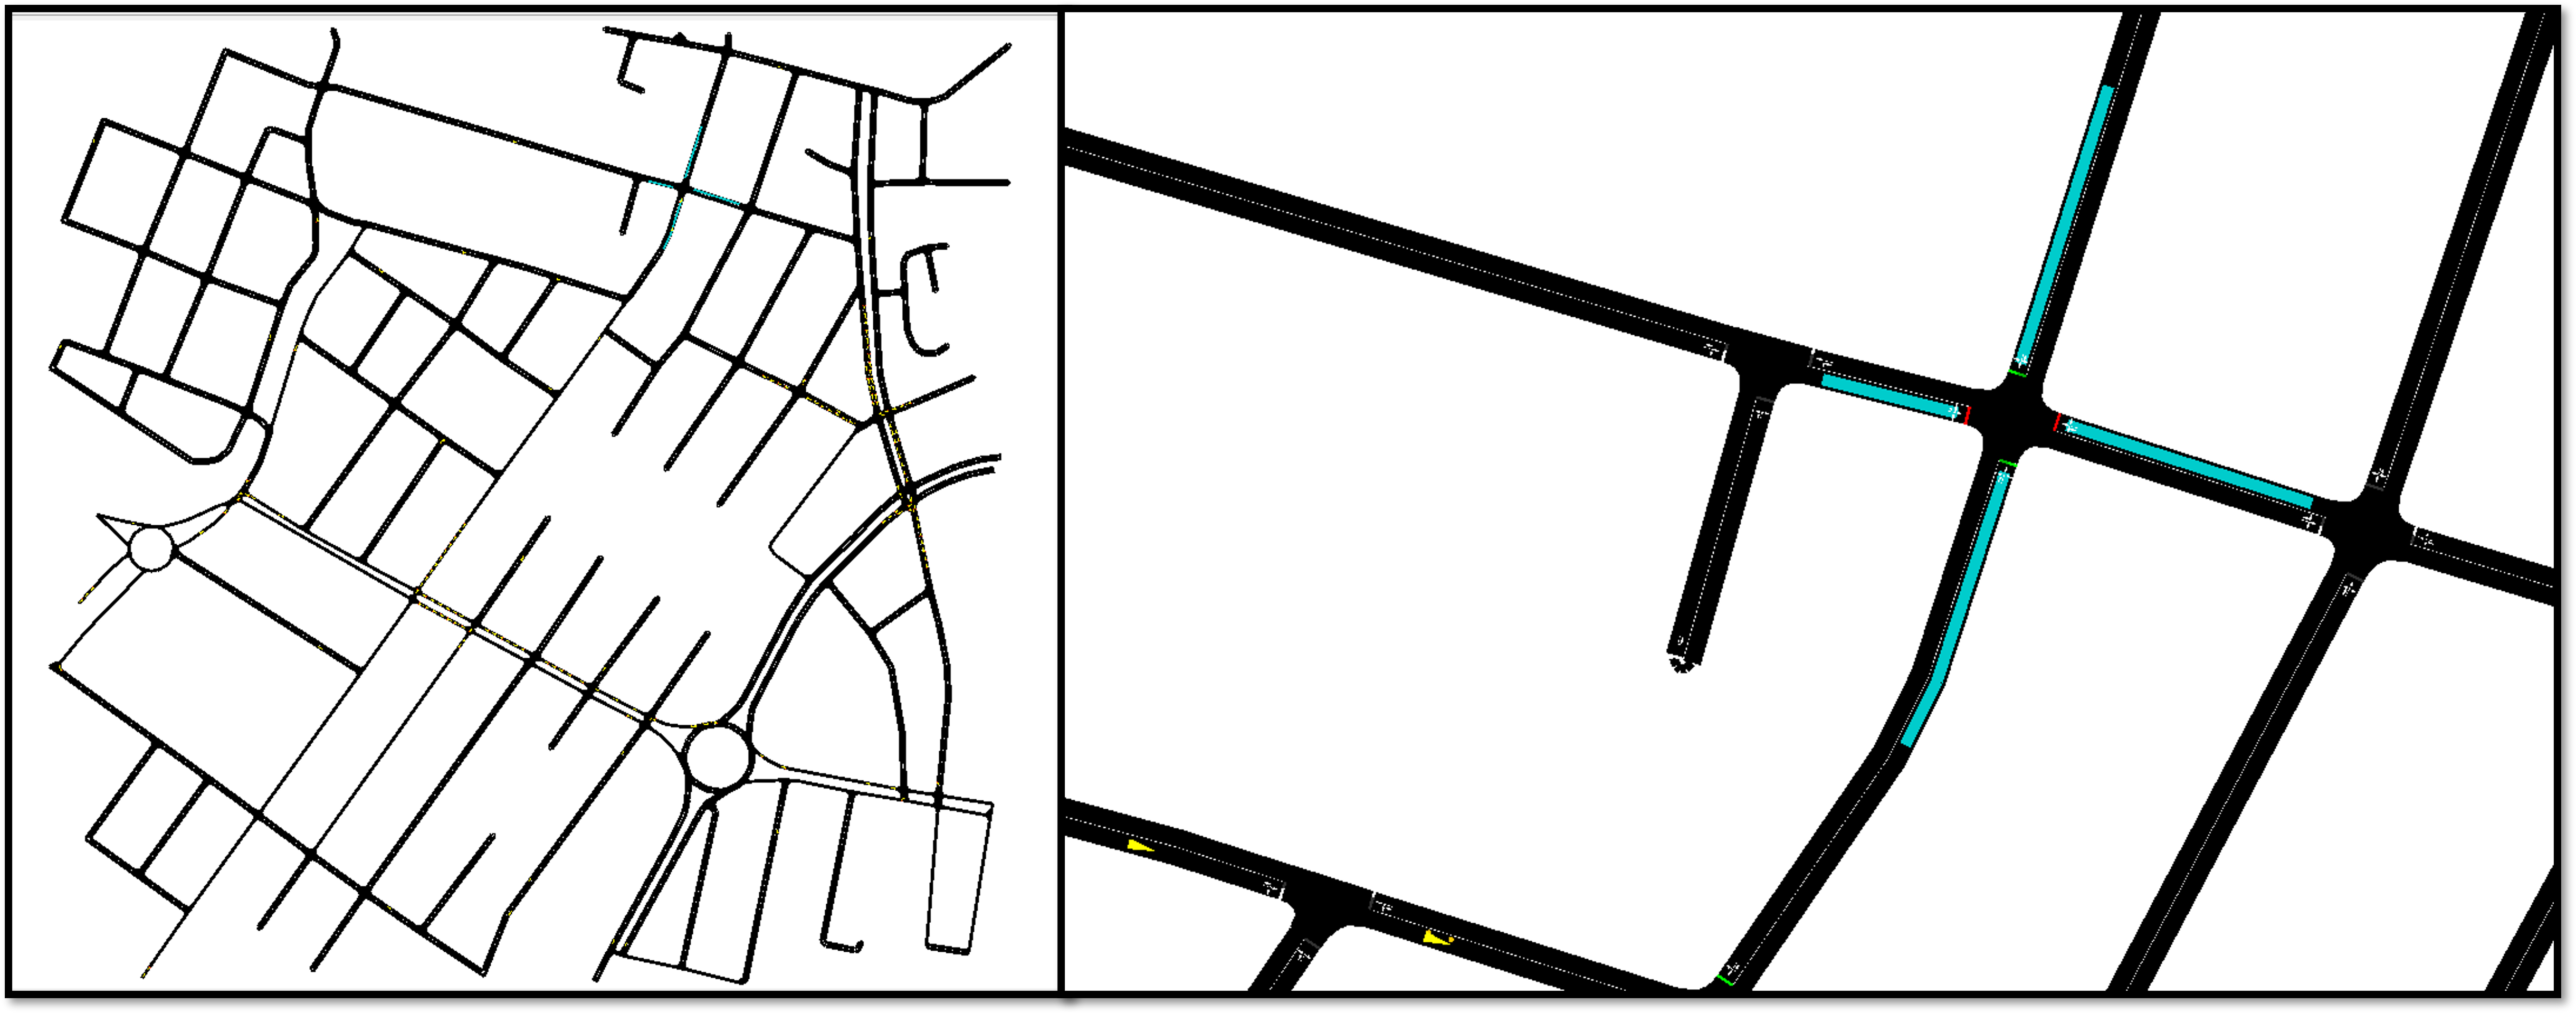
\includegraphics[width=0.9\textwidth]{images/mapa.png}
    \caption{Mapa de la zona de estudio: intersección del Mercado Mayorista. Se ilustra la geometría de la red y la disposición de los sensores en los accesos Norte, Sur, Este y Oeste.}
    \label{fig:mapa_zona}
\end{figure}

\section{Desempeño bajo Saturación Crítica (2000 veh/h)}
Uno de los hallazgos más relevantes de esta investigación fue identificar un rango crítico de operación del agente DRL. Mientras que en flujos bajos ambos sistemas se comportan de manera similar, y en saturación extrema la red colapsa físicamente, existe una zona de operación donde la inteligencia artificial marca una diferencia sustancial.

\begin{figure}[H]
    \centering
    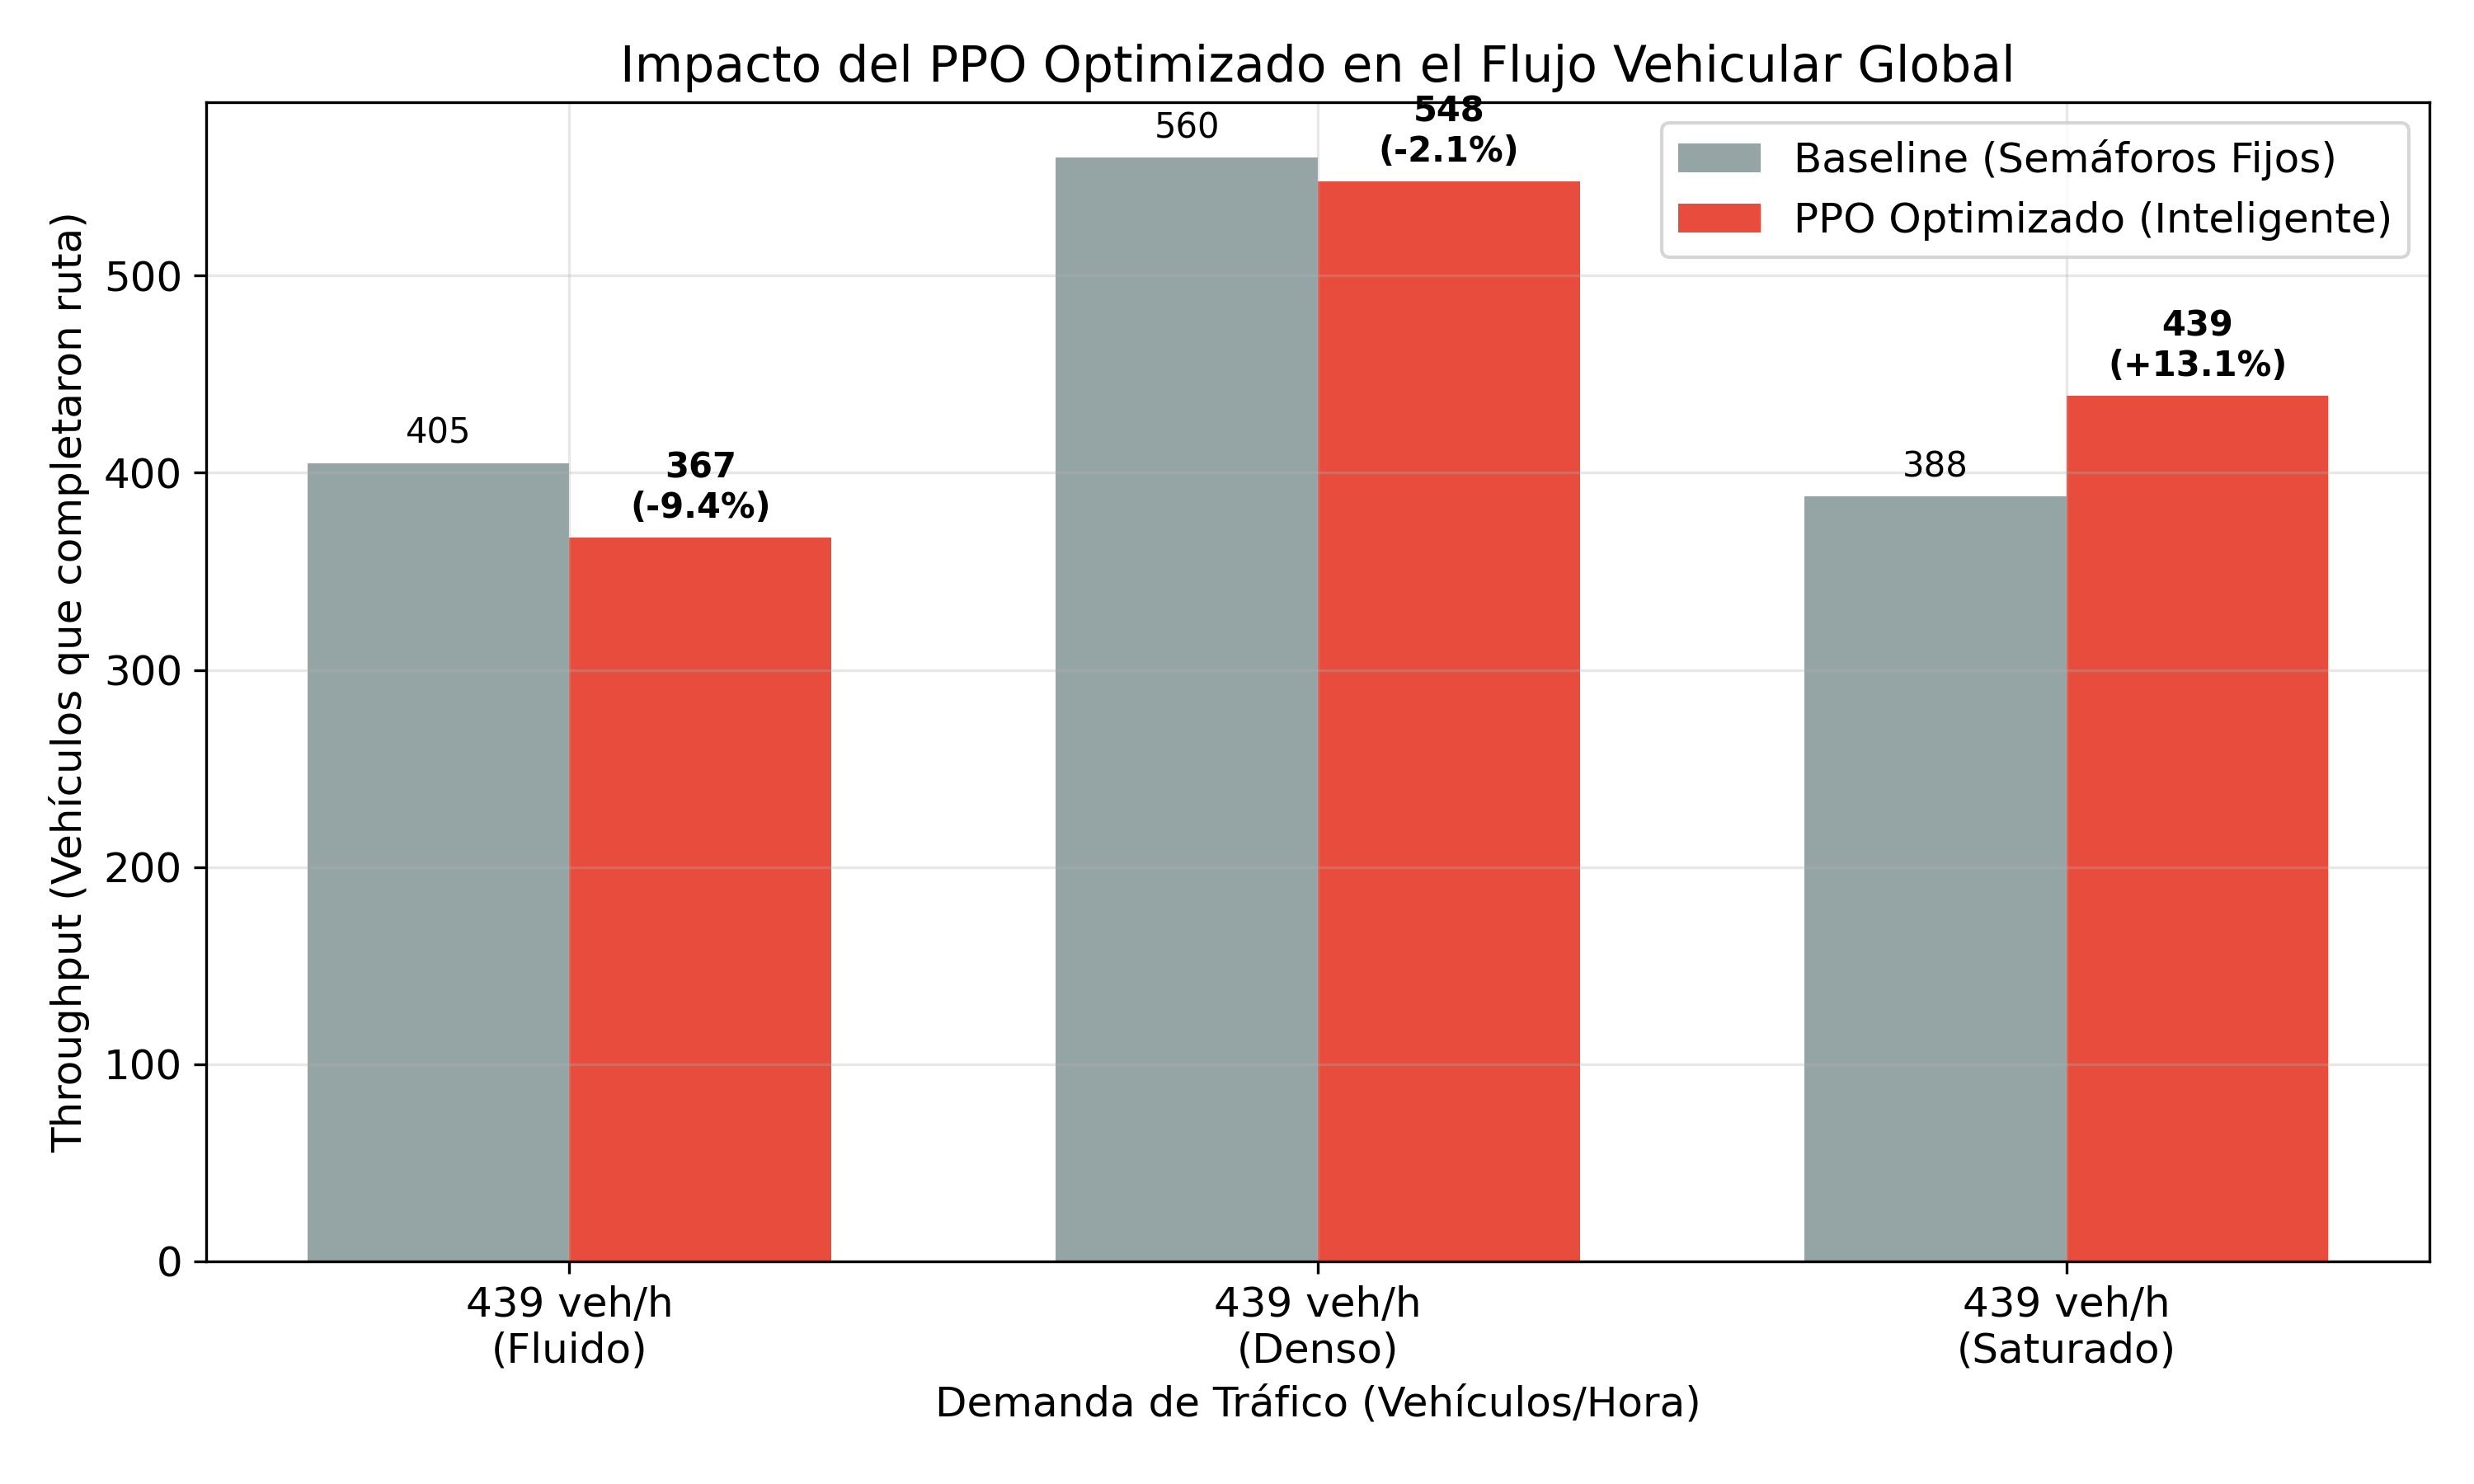
\includegraphics[width=0.8\textwidth]{images/throughput_comparison.png}
    \caption{Comparación de throughput acumulado en escenario de saturación (2000 veh/h).}
    \label{fig:throughput_saturacion}
\end{figure}

Como se evidencia en la Figura \ref{fig:throughput_saturacion}, bajo una carga sostenida de 2000 vehículos por hora durante el periodo de prueba extendido, el agente PPO logra procesar un volumen significativamente mayor de tráfico.

La mejora no solo es absoluta, sino porcentual. La Figura \ref{fig:relative_improvement} cuantifica esta ganancia.

\begin{figure}[H]
    \centering
    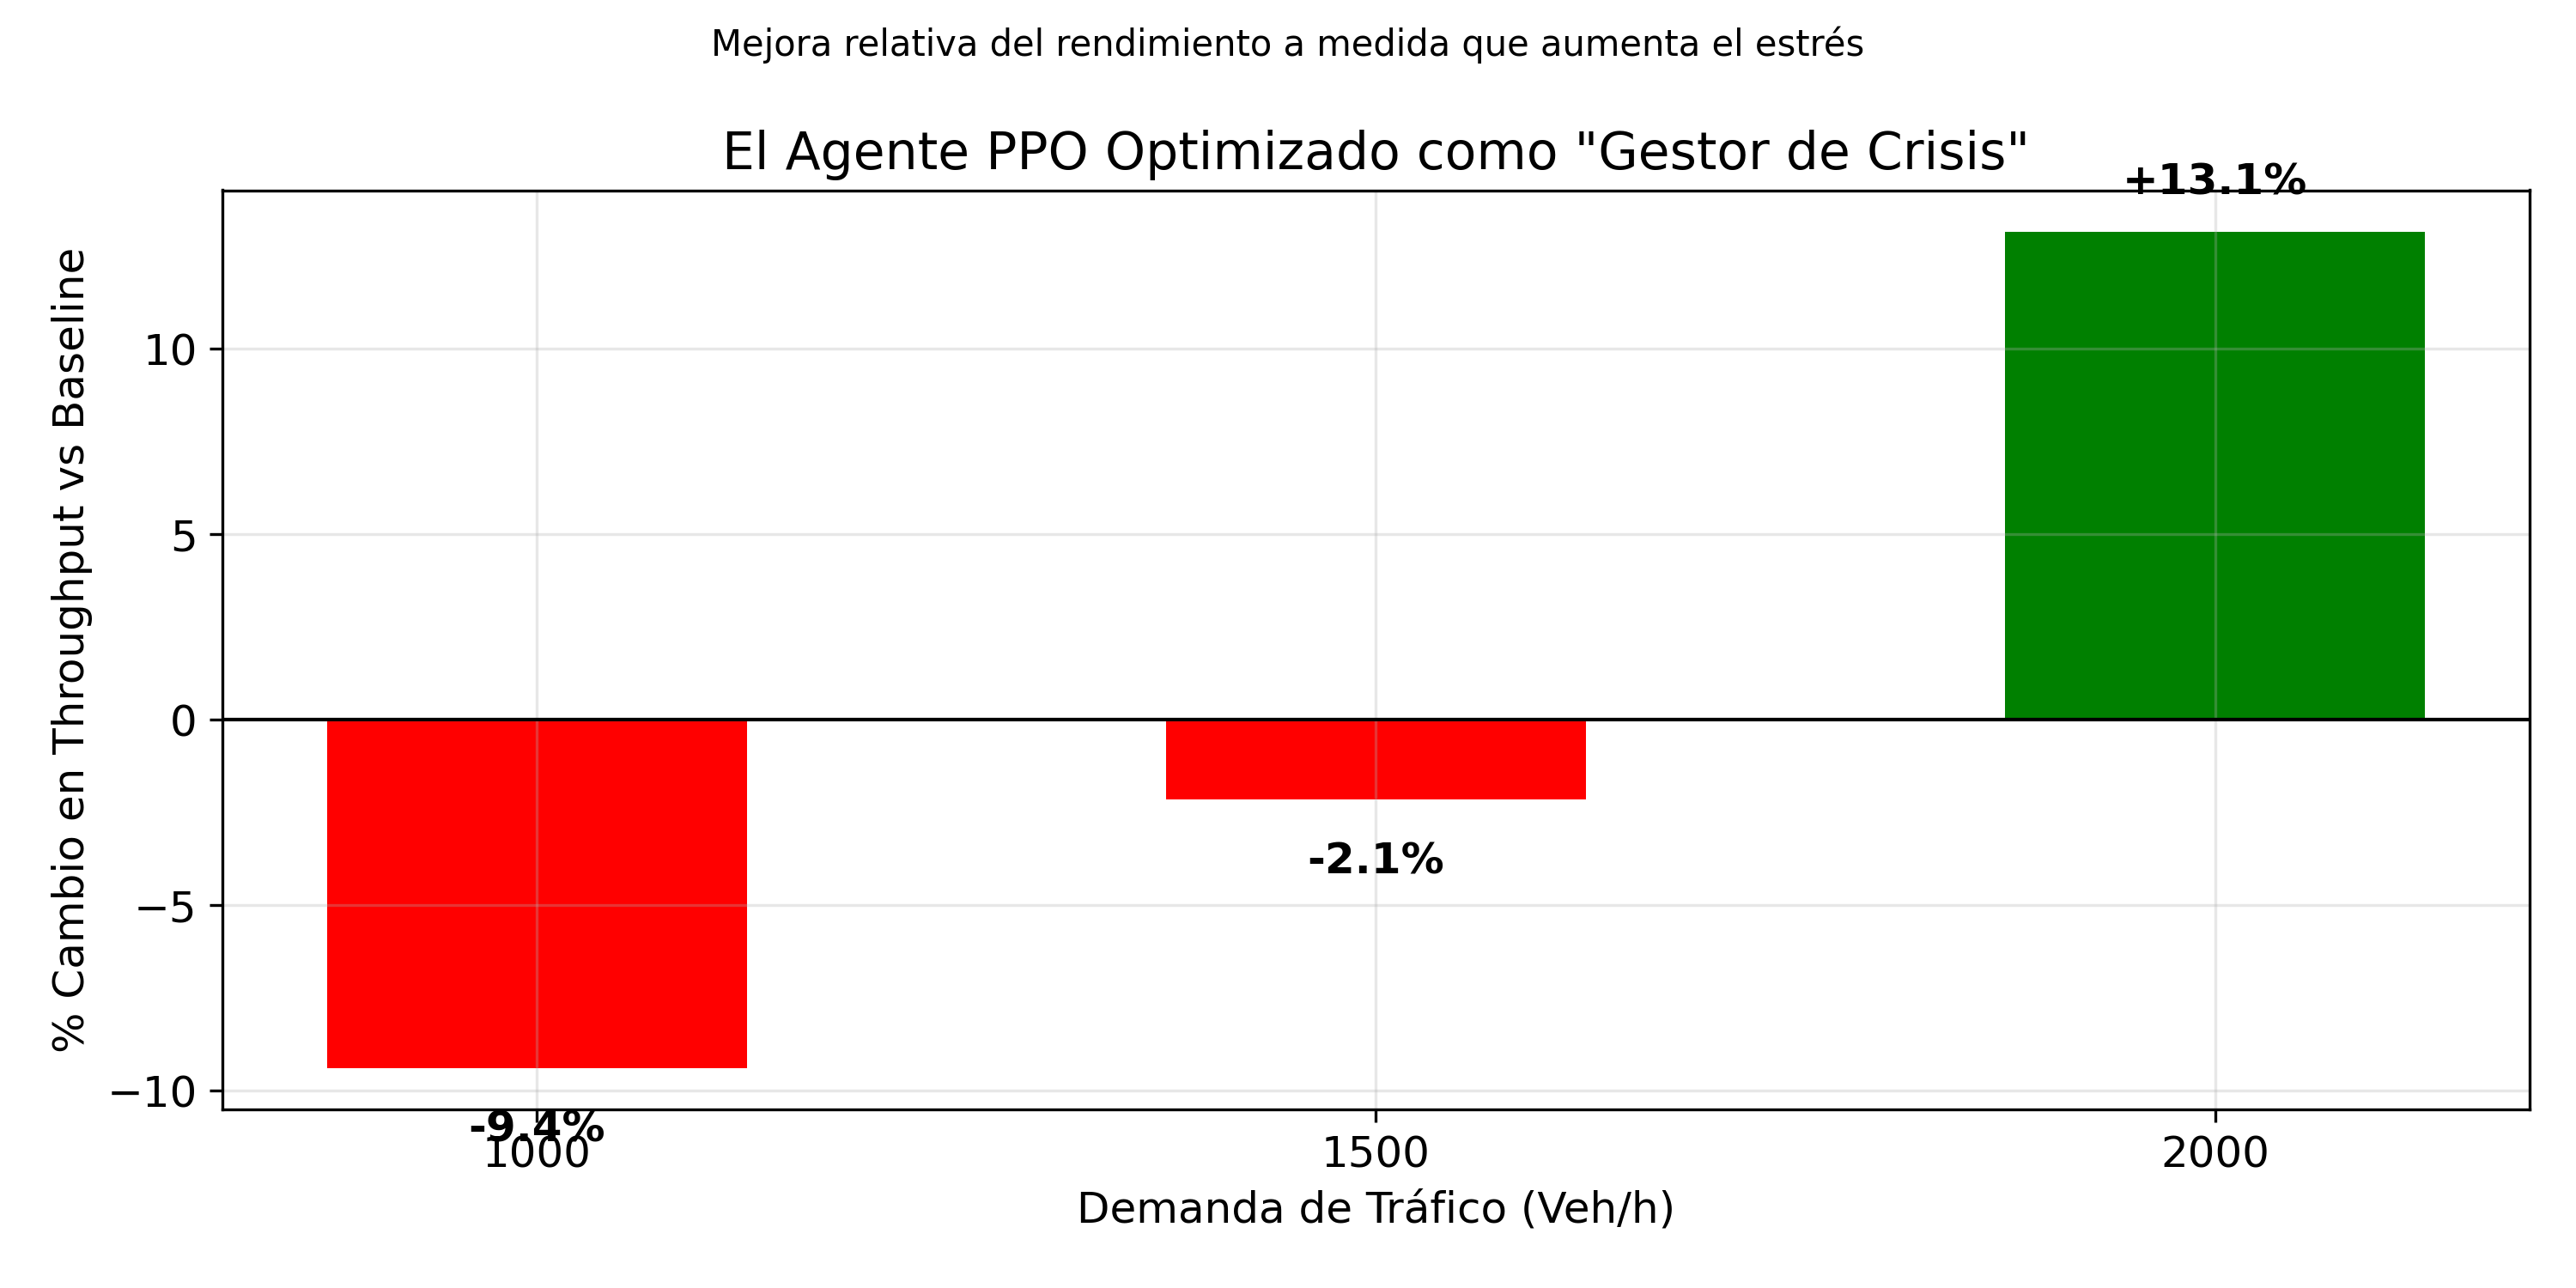
\includegraphics[width=0.8\textwidth]{images/relative_improvement.png}
    \caption[Mejora relativa porcentual del DRL frente al Baseline.]{Mejora relativa porcentual del DRL frente al Baseline. Se destaca una ganancia del \textbf{13.1\%} en la métrica de eficiencia de flujo.}
    \label{fig:relative_improvement}
\end{figure}

\noindent\textit{Nota:} La mejora relativa se calculó como el incremento en throughput acumulado $(T_{DRL} - T_{Baseline}) / T_{Baseline}$ al finalizar el periodo de evaluación bajo demanda constante de 2000 veh/h.

Este incremento del 13.1\% es crítico en ingeniería de tráfico, ya que representa la diferencia entre una vía funcional y una colapsada. Esta eficiencia superior se explica por la gestión de la congestión, mostrada en la Figura \ref{fig:congestion_levels}.

\begin{figure}[H]
    \centering
    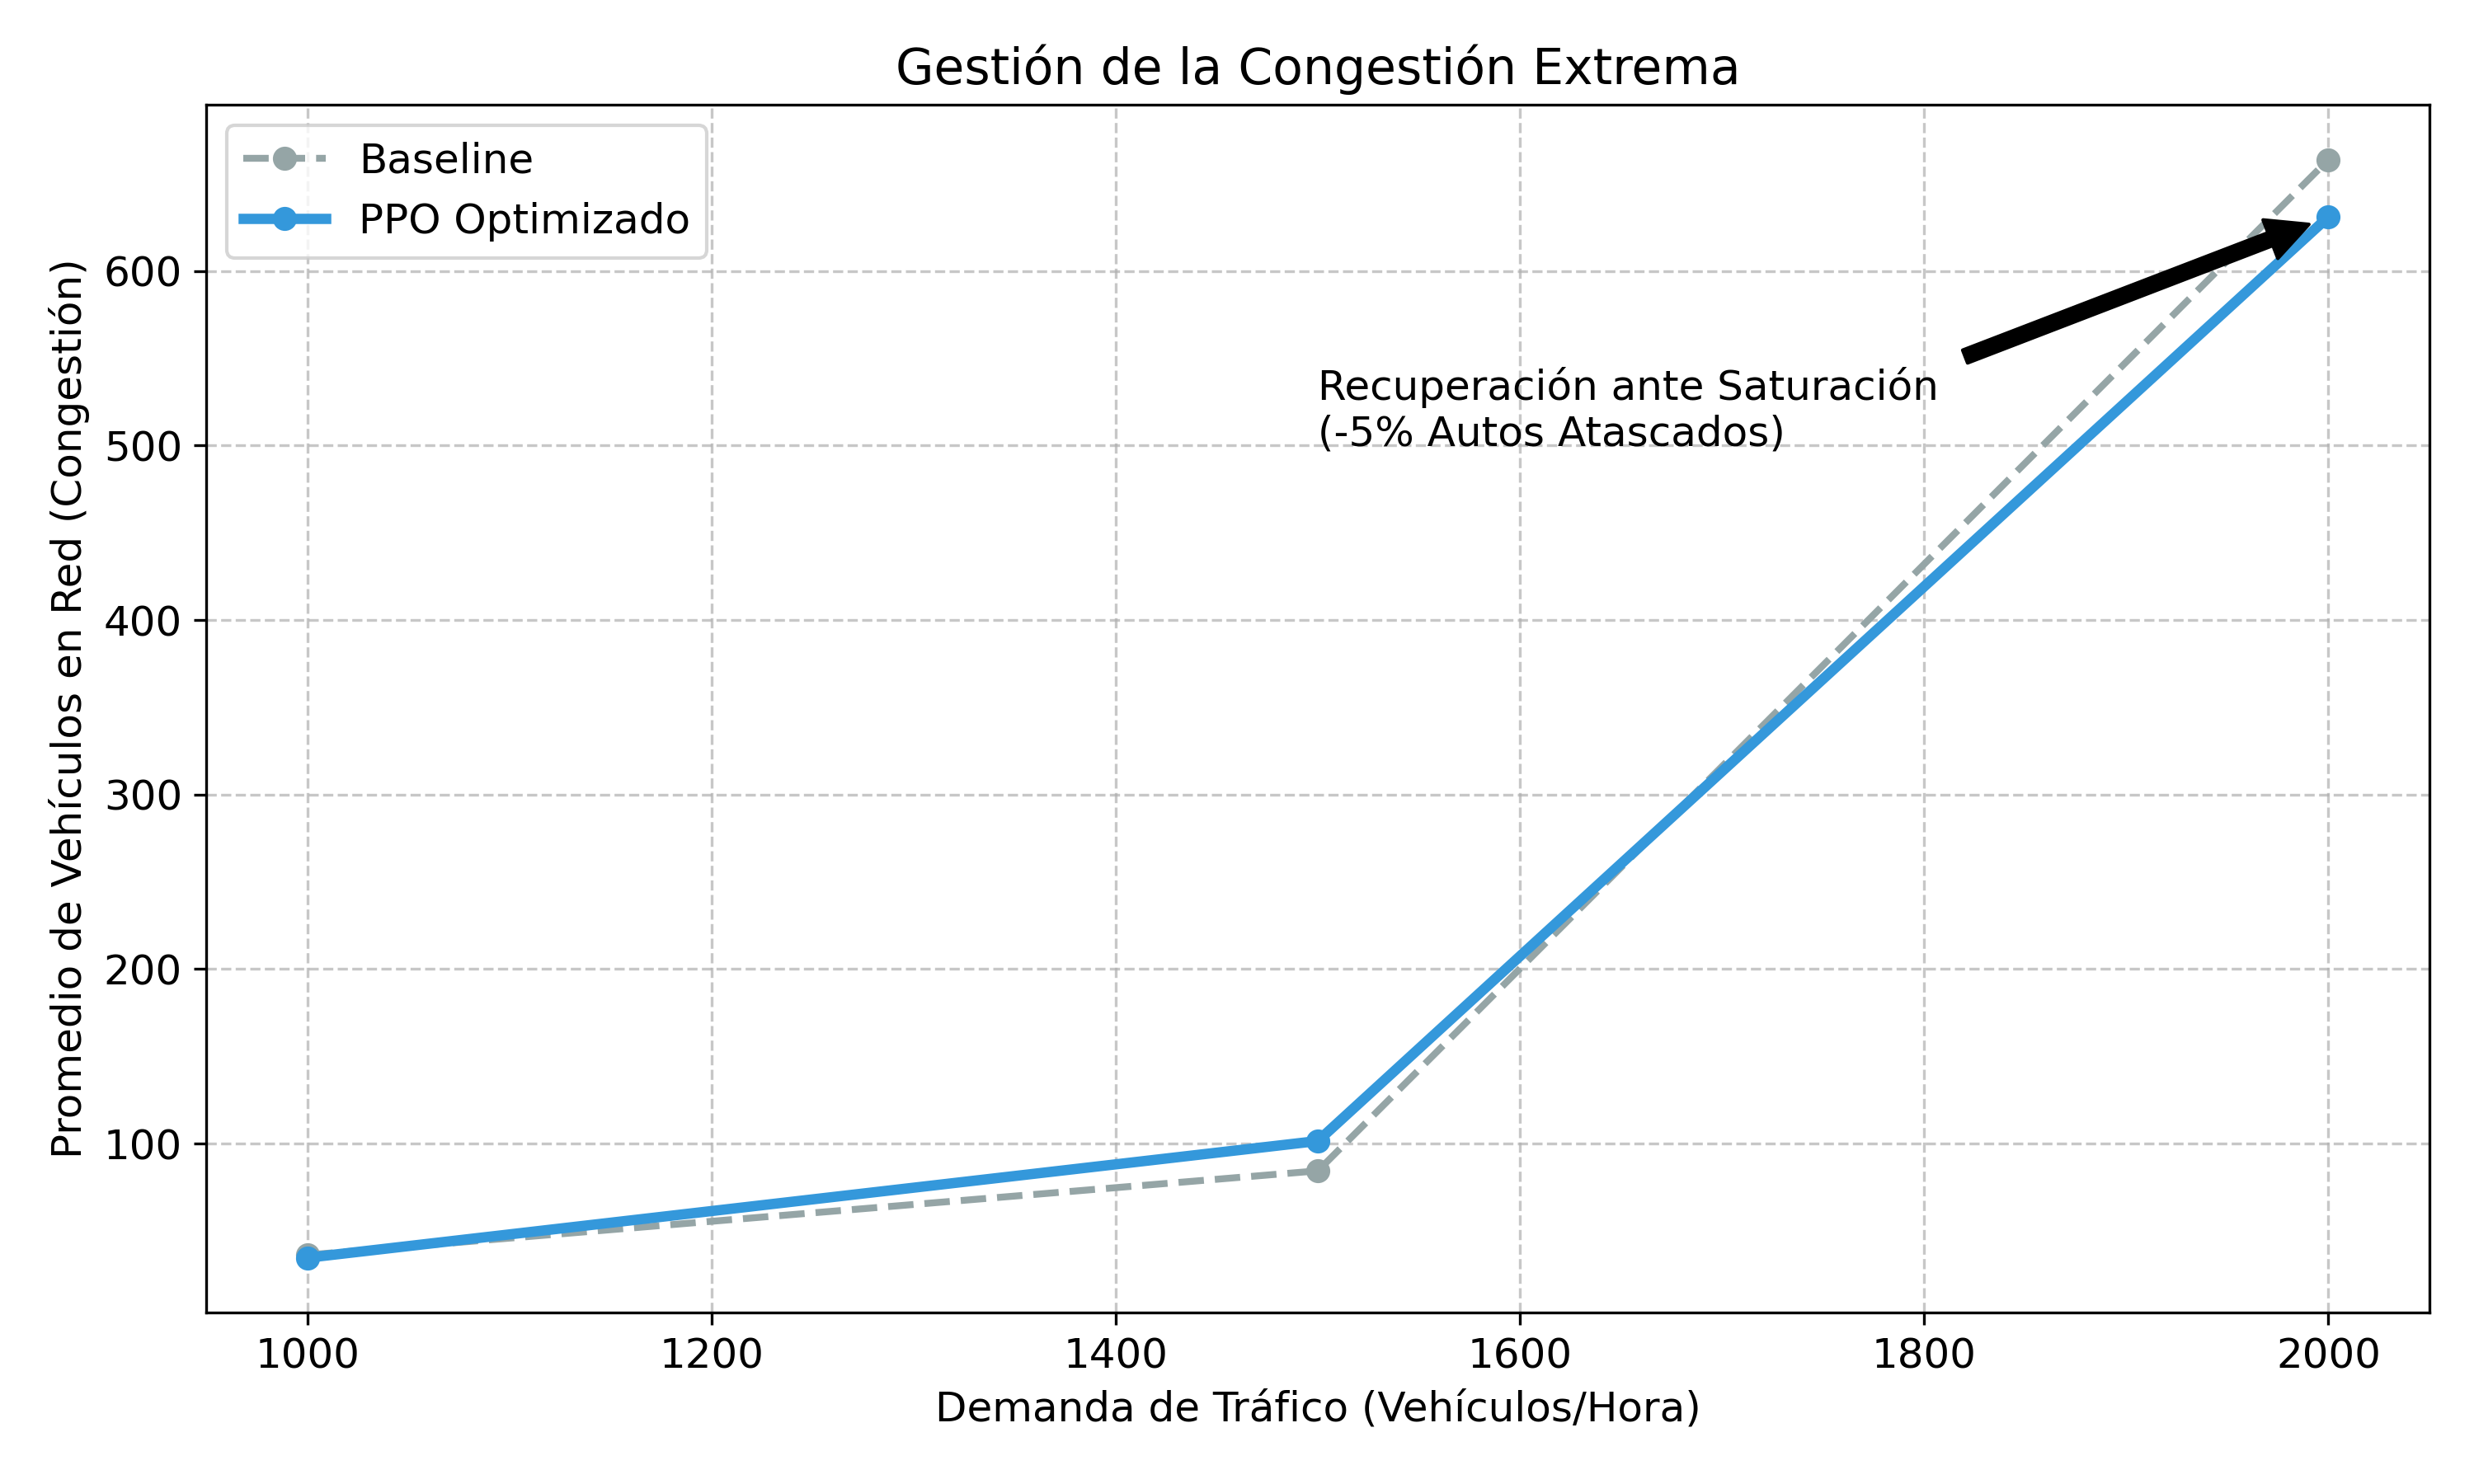
\includegraphics[width=0.8\textwidth]{images/congestion_levels.png}
    \caption{Niveles de congestión (vehículos detenidos) a lo largo del tiempo.}
    \label{fig:congestion_levels}
\end{figure}

El agente mantiene los niveles de congestión controlados, evitando el efecto acumulativo que se observa en el control de tiempo fijo, donde las colas remanentes de un ciclo obstruyen el siguiente.

\section{Análisis de sensibilidad del reward}
Durante el desarrollo, se observó que el diseño de la recompensa es crítico:

\begin{itemize}
    \item \textbf{Sin penalización de desequilibrio ($w_{unbalance}=0$):} El agente tendía a caer en políticas de hold infinito, dejando una fase en rojo durante periodos excesivos si el flujo entrante era constante.
    \item \textbf{Sin costo de cambio ($w_{switch}=0$):} El agente oscilaba rápidamente, lo cual es inseguro.
\end{itemize}
La combinación final de pesos ($w_{queue}=1.0, w_{unbalance}=0.2, w_{switch}=5.0$) logró el equilibrio deseado entre eficiencia y seguridad.
